En lo que sigue, se considerarán sistemas de la forma:
\begin{equation}
	\begin{aligned}
		\mathbf{x}_{k+1} &= \mathbf{f}(\mathbf{x}_k, \mathbf{w}_k), \\
		\mathbf{y}_k &= \mathbf{g}(\mathbf{x}_k, \mathbf{v}_k).
	\end{aligned}
	\label{eq:no_lin_dis_chap3}
\end{equation}
En comparación con el problema original, se omitirán explícitamente el tiempo y la entrada (\textit{input}) en la dinámica del sistema. Sin embargo, esto no implica una pérdida de generalidad. Por un lado, el tiempo puede ser incorporado como una variable de estado adicional, de manera que si se define \( \mathbf{x}_{k}^{n+1} = t_k \), entonces la evolución de esta coordenada viene dada por:
\begin{equation*}
    \mathbf{x}_{k+1}^{n+1} = \mathbf{x}_{k}^{n+1} + \Delta t_k,
\end{equation*}
donde \( \Delta t_k \) representa el paso de tiempo en el instante \( k \), el cual, en muchas aplicaciones, se asume constante.

Por otro lado, dado que la entrada \( \mathbf{u}_k \) no se considera una variable de decisión, se asumirá conocida o accesible de manera indefinida, es decir, la secuencia \( \{ \mathbf{u}_k \}_{k \geq 0} \) es completamente observable. En consecuencia, es suficiente con incorporarla como una coordenada adicional en el estado, es decir, \( \mathbf{x}_{k}^{n+1} = \mathbf{u}_k \).

El objetivo de este capítulo es presentar un marco general para el \textit{Kernel Extended Dynamic Mode Decomposition} (kEDMD) que se ajuste a los requerimientos previamente discutidos en la sección anterior. En particular, estos requerimientos incluyen:
\begin{itemize}
    \item La existencia de una función de \textit{lifting forward} que permita realizar un \textit{embedding} en un espacio de dimensión superior.
    \item Un operador que modele la evolución del sistema en tiempo discreto dentro del espacio embebido.
    \item Un operador de reconstrucción que posibilite la recuperación de las variables originales desde el espacio embebido.
    \item La representación de las observaciones en un espacio funcional de dimensión infinita.
\end{itemize}

La metodología propuesta establece una conexión entre los operadores de covarianza introducidos en los preliminares y el operador de Koopman, entendiendo este último como una herramienta más universal y transversal dentro del desarrollo del trabajo.

Finalmente, se enunciará y demostrará un teorema que cuantifica el error de aproximación del operador de Koopman en el contexto de los RKHS. Dicho resultado será utilizado posteriormente y comparado con el demostrado por Philipp et al. \cite{Philipp2024ErrorOperator}. Además, el mismo grupo de investigación ha desarrollado cotas de error en distintos contextos, lo que resulta relevante para futuras extensiones de este trabajo \cite{Philipp2023ErrorFramework, Nuske2023Finite-DataControl, Kohne2024L-errorDecomposition, Harder2024Group-ConvolutionalDecomposition, Philipp2024VarianceOperators, Peitz2025EquivarianceEquations}.

Es importante destacar que todas las construcciones presentadas en este capítulo, junto con el enfoque de formular el operador de Koopman como una herramienta transversal en el contexto de filtrado, así como la integración de cotas de error provenientes de la literatura, constituyen una contribución original de este trabajo.

\section{Operadores de Koopman en RKHS}

Sea $\B_\X$ la $\sigma$-álgebra de Borel definida sobre $\X$ y $\B_{\R^p}$ la correspondiente a $\R^p$. Se introducen las siguientes medidas de probabilidad:  
\[
\begin{aligned}
    \rho_f: \X \times \B_\X \to [0, 1], & \quad \rho_f (\mathbf{x}, A) = \P (\mathbf{f}(\mathbf{x}, \cdot ) \in A ), \\
    \rho_g: \X \times \B_\Y \to [0, 1], & \quad \rho_g(\mathbf{x}, A) = \P (\mathbf{g}(\mathbf{x}, \cdot ) \in A).
\end{aligned}
\]

En este contexto, $\rho_f$ representa la medida inducida por la dinámica del sistema, mientras que $\rho_g$ corresponde a la medida inducida por las observaciones.  
Se asume que el espacio de estados $\X$ es compacto con frontera Lipschitz y que existe un conjunto compacto $\Y \subseteq \R^p$ con frontera Lipschitz tal que  
\[
\rho_f (\mathbf{x}, \X) = 1, \quad \rho_g (\mathbf{x}, \Y) = 1, \quad \forall \mathbf{x} \in \X.
\]

Sea entonces $\B_\Y$ la $\sigma$-álgebra $\B_{\R^p}$ restringida a $\Y$. Se introduce la siguiente notación diferencial:
\[
\rho_f (\mathbf{x}, dx) = d \rho_f (\mathbf{x}, \cdot)(x), \quad \rho_g (\mathbf{x}, dy) = d \rho_g (\mathbf{x}, \cdot)(y).
\]
Adicionalmente, se consideran funciones de densidad  
\[
p_f : \X \times \X \to \R_+, \quad p_g : \X \times \Y \to \R_+,
\]
tales que, para $\mu_\X$ y $\mu_\Y$ medidas sobre $\X$ y $\Y$, respectivamente, se cumple:
\[
\rho_f (\mathbf{x}, A) = \int_A p_f (\mathbf{x}, y) \, d \mu_\X (y), \quad \rho_g (\mathbf{x}, A) = \int_A p_g (\mathbf{x}, y) \, d \mu_\Y (y).
\]

Bajo este marco, se adoptan las siguientes convenciones:
\begin{itemize}
    \item La variable aleatoria asociada a $\mu_\X$ se denota por $X$.  
    \item La variable aleatoria asociada a $\rho_f$, que describe la evolución de un estado $\mathbf{x}$ tras un paso de la dinámica, se denota por $X^+ \mid \mathbf{x}$.  
    \item La variable aleatoria asociada a $\rho_g$, que modela las observaciones condicionadas a un estado $\mathbf{x}$, se denota por $Y \mid \mathbf{x}$.  
\end{itemize}

\begin{obs}
Un ejemplo concreto de este marco es el siguiente: considérese el caso en que la dinámica del sistema está dada por  
\[
    \mathbf{f}(\mathbf{x}_k, \mathbf{w}_k) = \Tilde{\mathbf{f}}(\mathbf{x}_k) + \mathbf{w}_k,
\]
donde $\mathbf{w}_k \sim \mathcal{N}(0, \mathbf{Q}_k)$, con $\mathbf{Q}_k$ definida positiva, y donde $\mu_\X$ es la medida de Lebesgue, normalizada, en $\X$. En este caso, la medida $\rho_f (\mathbf{x}_k, \cdot)$ sigue una distribución normal:  
\[
    \rho_f (\mathbf{x}_k, \cdot) \sim \mathcal{N}(\Tilde{\mathbf{f}}(\mathbf{x}_k), \mathbf{Q}_k).
\]
    
En consecuencia, la densidad $p_f$ asociada toma la forma  
\[
p_f(x, y) = (2 \pi \det \mathbf{Q}_k )^{-1/2} \exp \left( -\frac{1}{2} (\Tilde{\mathbf{f}}(x) - y)^\top \mathbf{Q}_k^{-1} (\Tilde{\mathbf{f}}(x) - y) \right).
\]
\end{obs}

Para garantizar la validez de los resultados en \cite{Philipp2024ErrorOperator}, se asumirán las siguientes hipótesis de compatibilidad:
\begin{enumerate}
    \item[a)] Sean $k_\X:\X \times \X \to \R$ y $k_\Y: \Y \times \Y \to \R$ dos \textit{kernels} simétricos, continuos, acotados y semi-definidos positivos. Se denotará por $\H_\X$ y $\H_\Y$ a los RKHS asociados a $k_\X$ y $k_\Y$, respectivamente.
    
    \item[b)] Si $\psi_\X \in L^2(\X)$ y $\psi_\Y \in L^2(\Y)$ satisfacen  
    \[
        \int_{\X \times \X} k_\X(x,y) \psi_\X (x) \psi_\X (y) d \mu_\X (x) d \mu_\X (y) = 0, 
    \]
    \[
        \int_{\Y \times \Y} k_\Y(x,y) \psi_\Y (x) \psi_\Y (y) d \mu_\Y (x) d \mu_\Y (y) = 0, 
    \]
    entonces $\psi_\X = 0$ y $\psi_\Y = 0$ casi seguramente.
    
    \item[c)] Si $\psi_\X \in \H_\X$ y $\psi_\Y \in \H_\Y$ son tales que $\psi_\X(x) = 0$ para todo $x \in \X$ $\mu_\X$-casi seguramente, y $\psi_\Y(y) = 0$ para todo $y \in \Y$ $\mu_\Y$-casi seguramente, entonces $\psi_\X \equiv 0$ y $\psi_\Y \equiv 0$.
    
    \item[d)] Se asumen las siguientes relaciones entre $\rho_f$ y $\rho_g$ con respecto a $\mu_\X$ y $\mu_\Y$:
    \[
        \int_\X \rho_f (x, A_\X) d\mu_\X (x) \leq L_\X \mu_\X (A_\X), \quad \forall A_\X \in \B_\X,
    \]
    \[
        \int_\X \rho_g (x, A_\Y) d\mu_\X (x) \leq L_\Y \mu_\Y (A_\Y), \quad \forall A_\Y \in \B_\Y.
    \]
\end{enumerate}

Un ejemplo de un \textit{kernel} que satisface las hipótesis a) y b) es el \textit{kernel} de Matérn. La propiedad a) es garantizada por los resultados presentados en la sección anterior, mientras que la propiedad b) se deriva de la universalidad del \textit{kernel} en $L^2$. 

La hipótesis c) se satisface si $\mu_\X$ y $\mu_\Y$ tienen densidad respecto a la medida de Lebesgue, y la hipótesis d) se cumple en el caso estocástico cuando las funciones $p_f$ y $p_g$ son acotadas, tal como se verá en la proposición a continuación.

\begin{prop}
    Si $p_f \in L^{\infty} (\X \times \X)$ y $p_g \in L^{\infty} (\X \times \Y)$, entonces:
    \[
        \int_\X \rho_f (x, A) d\mu_\X (x) \leq L_\X \mu_\X (A), \quad \int_\X \rho_g (x, A) d\mu_\X (x) \leq L_\Y \mu_\Y (A),
    \]
    donde:
    \[
        L_\X = \mu_\X (\X) \| p_f \|_\infty, \quad L_\Y = \mu_\X (\X) \| p_g \|_\infty.
    \]
\end{prop}

\begin{proof}
    Para $\rho_f$, se tiene que:
    \[
        \begin{aligned}
            \int_\X \rho_f (x, A) d\mu_\X (x) &= \int_\X \int_A d \rho_f (x, \cdot) (y) d \mu_\X (x) \\
            &= \int_\X \int_A p_f (x, y) d \mu_\X (y) d \mu_\X (x) \\
            &\leq \| p_f \|_\infty \int_\X \int_A d \mu_\X (y) d \mu_\X (x) \\ 
            &= \| p_f \|_\infty \mu_\X (\X) \mu_\X (A) \\
            &= L_\X \mu_\X (A).
        \end{aligned}
    \]
Para $\rho_g$, de manera similar, se tiene que:
    \[
        \begin{aligned}
            \int_\X \rho_g (x, A) d\mu_\X (x) &= \int_\X \int_A d \rho_g (x, \cdot) (y) d \mu_\X (x) \\
            &= \int_\X \int_A p_g (x, y) d \mu_\Y (y) d \mu_\X (x) \\
            &\leq \| p_g \|_\infty \int_\X \int_A d \mu_\Y (y) d \mu_\X (x) \\ 
            &= \| p_g \|_\infty \mu_\X (\X) \mu_\Y (A) \\
            &= L_\Y \mu_\Y (A).
        \end{aligned}
    \]
\end{proof}
En el caso en que la dinámica y la observación sean deterministas, esto es equivalente a que $\mathbf{f}(\mathbf{x}, \mathbf{w}) = \Tilde{\mathbf{f}}(\mathbf{x})$ y $\mathbf{g}(\mathbf{x}, \mathbf{v}) = \Tilde{\mathbf{g}}(\mathbf{x})$, con lo que $\rho (x, \cdot) = \delta_{\Tilde{\mathbf{f}}(x)}(\cdot)$ y $\xi (x, \cdot) = \delta_{\Tilde{\mathbf{g}}(x)}(\cdot)$ y por tanto no se satisfacen las hipótesis de la proposición anterior. En este caso, es necesario asumir mayor regularidad sobre las funciones involucradas.

\begin{prop}
    Si $\rho (x, \cdot) = \delta_{\Tilde{\mathbf{f}}(x)}(\cdot)$ y $\xi (x, \cdot) = \delta_{\Tilde{\mathbf{g}}(x)}(\cdot)$, y $\tilde{\mathbf{f}}$ y $\tilde{\mathbf{g}}$, según corresponda, son difeomorfismos de clase $C^1$ tales que:
    \begin{equation*}
        \inf_{x \in \X} \left | \det ( D \tilde{\mathbf{f}} (x) ) \right | > 0, \quad \inf_{x \in \X} \left | \det ( D \tilde{\mathbf{g}} (x) ) \right | > 0,
    \end{equation*}
    entonces:
    \begin{equation*}
        \int_\X \rho_f (x, A) d\mu (x) \leq L_f \mu (A), \quad \int_\X \rho_g (x, A) d\mu_\X (x) \leq L_g \mu_\Y (A),
    \end{equation*}
    con:
    \begin{equation*}
        L_f = \left \| \det ( D \tilde{\mathbf{f}}^{-1} ) \right \|_\infty, \quad L_g = \left \| \det ( D \tilde{\mathbf{g}}^{-1} ) \right \|_\infty.
    \end{equation*}
\end{prop}
\begin{proof}

La demostración sigue un razonamiento similar al expuesto en \cite{Kohne2024L-errorDecomposition}. Para un conjunto $A \in \B$, se observa que $\rho_f (x, A) = \delta_{\Tilde{\mathbf{f}}(x)}(A) = \mathds{1}_A (\Tilde{\mathbf{f}}(x))$. Por lo tanto:
\begingroup
\allowdisplaybreaks
    \begin{equation*}
        \begin{aligned}
            \int_\X \rho_f (x, A) d\mu (x) &= \int_\X \mathds{1}_A (\Tilde{\mathbf{f}}(x)) d \mu_\X (x) \\
            &= \int_\X \mathds{1}_A (x) \left | \det ( D \Tilde{\mathbf{f}}^{-1}(x) ) \right | d \mu_\X (x) \\
            &\leq \left \| \det ( D \Tilde{\mathbf{f}}^{-1} ) \right \|_\infty \int_\X \mathds{1}_A (x) d\mu_\X (x) \\
            &= \left \| \det ( D \Tilde{\mathbf{f}}^{-1} ) \right \|_\infty \mu_\X (A) \\
            &= L_f \mu_\X (A).
        \end{aligned}
    \end{equation*}
\endgroup
    El caso de $\rho_g$ se demuestra de manera análoga.
\end{proof}

A continuación, se presentan las definiciones de los operadores de Koopman estocásticos para la dinámica y la observación, adaptados al caso en que se disponen de las funciones $p_f$ y $p_g$ como densidades.

\begin{defn}[Operador de Koopman estocástico para la dinámica, tiempo discreto]
	Se define el operador asociado a $\mathbf{f}$ como $\U : L^2(\X) \to L^2(\X)$, dado por:
	\begin{equation*}
		[\U h](x) = \E [h (\mathbf{f} (x, \cdot) )]  = \int_\X h(x') \rho_f (x, dx') = \int_\X h(x') p_f (x, x') d \mu_\X (x').
	\end{equation*}
\end{defn}

\begin{defn}[Operador de Koopman estocástico para la observación]
    Se define el operador asociado a $\mathbf{g}$ como $\G : L^2(\Y) \to L^2(\X)$, dado por:
	\begin{equation*}
		[\G h](x) = \E [h (\mathbf{g} (x, \cdot) )]  = \int_\Y h(y) \rho_g (x, dy) = \int_\Y h(y) p_g (x, y) d \mu_\Y (y).
	\end{equation*}
\end{defn}

Se introduce el operador de Perron-Frobenius, que posteriormente mostrará no solo una relación con el operador de Koopman, sino también la dinámica subyacente. A continuación, se presentan sus definiciones en el contexto estocástico para la dinámica y la observación.

\begin{defn}[Operador de Perron-Frobenius estocástico para la dinámica]
	Se define el operador asociado a $\mathbf{f}$ como $\mathcal{P}_\mathbf{f} : L^2(\X) \to L^2(\X)$, dado por:
	\begin{equation*}
		[\mathcal{P}_\mathbf{f} h](x) = \int_\X h(x') p_f (x', x) d \mu_\X (x').
	\end{equation*}
\end{defn}

\begin{defn}[Operador de Perron-Frobenius estocástico para la observación]
	Se define el operador asociado a $\mathbf{g}$ como $\mathcal{P}_\mathbf{g} : L^2(\X) \to L^2(\Y)$, dado por:
	\begin{equation*}
		[\mathcal{P}_\mathbf{g} h](x) = \int_\X h(y) p_g (y, x) d \mu_\X (y).
	\end{equation*}
\end{defn}

Dado que los operadores $\mathcal{P}_\mathbf{f}$ y $\mathcal{P}_\mathbf{g}$ están definidos en términos de las funciones de densidad $p_f$ y $p_g$, se cumple que:
\begin{equation*}
	\U^* = \mathcal{P}_\mathbf{f}, \quad \G^* = \mathcal{P}_\mathbf{g},
\end{equation*}
donde $\U^*$ y $\G^*$ denotan los operadores adjuntos de $\U$ y $\G$, respectivamente.

En este punto se tomará la elección de tomar $k_\Y$ como el \textit{kernel} dado por el producto interno en $\R^p$, con lo que su \textit{feature map} canónico es la función identidad en dicho espacio y $\H_\Y = (\R^p)^*$, que dado que es isométricamente isomorfo a $\R^p$, se considerará como este último cuando sea conveniente. En lo que sigue, se retomarán las definiciones de la sección anterior, pero específicas en este contexto.

\begin{defn}[Feature map canónico]
	Se definen los \textit{feature maps} canónicos de los \textit{kernels} $\Phi_\X : \X \to \H_\X$ y $\Phi_\Y : \Y \to \R^p$ como:
	\begin{equation*}
		\Phi_\X (x) = k_\X (x, \cdot), \quad \Phi_\Y (y) = k_\Y (y, \cdot) = \langle y, \cdot \rangle.
	\end{equation*}
\end{defn}

\begin{defn}
	Para $x_1, x_2 \in \X$ y $y_1, y_2 \in \Y$, se definen los operadores de rango 1 $C_{x_1,x_2} : \H_\X \to \H_\X$, $C_{y_1,y_2} : \R^p \to \R^p$ y $C_{y_1,x_1} : \H_\X \to \R^p$ como:
	\begin{equation*}
		C_{x_1, x_2} \psi = \langle \psi, \Phi_\X (x_2) \rangle \Phi_\X (x_1) = \psi (x_2) \Phi_\X (x_1),
	\end{equation*}
	\begin{equation*}
		C_{y_1, y_2} \psi = \langle \psi, \Phi_\Y (y_2) \rangle \Phi_\Y (y_1) = \psi (y_2) \Phi_\Y (y_1),
	\end{equation*}
	\begin{equation*}
		C_{y_1, x_1} \psi = \langle \psi, \Phi_\X (x_1) \rangle \Phi_\Y (y_1) = \psi (x_1) \Phi_\Y (y_1).
	\end{equation*}
\end{defn}

\begin{defn}[Operadores de covarianza]
	Se definen los operadores de covarianza 
    \begin{equation*}
        C_X : \H_\X \to \H_\X, \quad C_Y : \R^p \to \R^p
    \end{equation*} 
    como:
	\begin{equation*}
		C_X \psi = \int_\X \langle \psi, \Phi_\X (x) \rangle \Phi_\X (x) d \mu_\X (x) = \int_\X [\Phi_\X (x) \otimes \Phi_\X (x)] \psi d \mu_\X (x),
	\end{equation*}
	\begin{equation*}
		C_Y \psi = \int_\Y \langle \psi, \Phi_\Y (y) \rangle \Phi_\Y (y) d \mu_\Y (y) = \int_\Y [\Phi_\Y (y) \otimes \Phi_\Y (y)] \psi d \mu_\Y (y).
	\end{equation*}
\end{defn}

\begin{defn}[Operadores de covarianza cruzada]
    El operador de covarianza cruzada asociado a la dinámica es $C_{X X^+} : \H_\X \to \H_\X$, dado por:
	\begin{equation*}
		C_{X X^+} \psi = \E[\Phi_\X (X) \otimes \Phi_\X (X^+)] \psi = \int_\X \int_\X \langle \psi, \Phi_\X (y) \rangle \Phi_\X (x) d\rho_f (x, \cdot)(y) d \mu_\X (x).
	\end{equation*}
    
    El operador de covarianza cruzada asociado a la observación es $C_{YX} : \H_\X \to \R^p$, dado por:
	\begin{equation*}
		C_{Y X} \psi = \E[\Phi_\Y (Y) \otimes \Phi_\X (X)] \psi = \int_\X \int_\Y \langle \psi, \Phi_\X (x) \rangle \Phi_\Y (y) d\rho_g (x, \cdot)(y) d \mu_\X (x).
	\end{equation*}
\end{defn}

\begin{defn}[Operadores de \textit{embedding} condicional]   
    Se definen los operadores de \textit{embedding} condicional $C_{X^+ | X} : \H_\X \to \H_\X$ y $C_{Y | X} : \H_\X \to \R^p$ como:
	\begin{equation*}
		C_{X^+ | X} = C_{X^+ X} C_X^{-1}, \quad C_{Y | X} = C_{Y X} C_X^{-1}.
	\end{equation*}
\end{defn}

Finalmente, será necesario asumir que $\U \H_\X \subset \H_\X$ y $\G (\R^p)^* \subset \H_\X$. Esto se cumple, por ejemplo, si $\H_\X$ es un espacio de Sobolev, como en el caso de que $k_\X$ sea un \textit{kernel} de Matérn. En este contexto, Köhne et al. \cite{Kohne2024L-errorDecomposition} prueban que esto se tiene cuando las funciones asociadas son difeomorfismos. A efectos de este trabajo fue necesario extender dicho resultado al caso estocástico, lo que se refleja en los siguientes dos resultados. Para la demostración será necesario un teorema de interpolación de espacios de Sobolev de Brenner y Scott \cite{Brenner2008TheMethods}.

\begin{lema}
    \label{lema:interpolacion}
    Sea $\X$ un compacto con frontera Lipschitz y $H^s(\X)$ el espacio de Sobolev asociado a $\X$ con integrabilidad $p=2$ y regularidad $s$, luego para $s, k > 0$ se tiene que
    \[
        H^{s+\theta \cdot k} (\X) = [H^s (\X), H^{s+k} (\X)]_\theta.
    \]
    En particular, si $\psi \in H^{s}(\X)$ y $\psi \in H^{s+k}(\X)$, entonces $\psi \in H^{s+\ell}$ para todo $\ell \in [0, k]$.
\end{lema}

\begin{prop}[Invarianza Sobolev para Koopman]
	Sea $s \geq 0$, $k =\lceil s \rceil $ y $H^s(\X)$ el espacio de Sobolev sobre $\X$. Si $p_f \in C^{k,k} (\X \times \X)$ y $p_g \in C^{k,k} (\X \times \Y)$, entonces:
	\begin{equation*}
		\U H^s (\X) \subseteq H^s (\X), \quad \G (\R^p)^* \subseteq H^s (\X).
	\end{equation*}
\end{prop}

\begin{proof}
	Sea $m \in \N$, $m \leq k$ y $|\alpha| = m$ un multiíndice. Para $h \in H^m (\X)$, por el teorema de la convergencia dominada:
	\begin{equation*}
		\partial^\alpha_x (\U h)(x) = \int_\X h(y) \partial^\alpha_x p_{\mathbf{f}} (x, y) d \mu_\X (y).
	\end{equation*}
	Por lo tanto:
	\begin{equation*}
		\begin{aligned}
			\| \partial^\alpha_x (\U h) \|_{L^2}^2 & \leq \int_\X \int_\X h(y)^2 \partial^\alpha_x p_{\mathbf{f}} (x, y)^2 d \mu_\X (y) d \mu_\X (x) \\
			& \leq \| \partial^\alpha_x p_{\mathbf{f}} \|_{C^{k,k}} \mu_\X (\X) \int_\X h(y)^2 d \mu_\X (y) \\
			& \leq \| \partial^\alpha_x p_{\mathbf{f}} \|_{C^{k,k}} \mu_\X (\X) \| h \|_{\H^k (\X)}^2.
		\end{aligned}
	\end{equation*}
	Así, se concluye que $\U h \in H^m (\X)$ y:
	\begin{equation*}
		\| \U \|_{H^m (\X) \to H^m (\X)} \leq \mu_\X (\X) \sum_{|\alpha| \leq k} \| \partial^\alpha_x p_{\mathbf{f}} \|_{C^{k,k}}.
	\end{equation*}
        Es así que
        \[
        \U H^m (\X) \subseteq H^m (\X), \, \forall m \in \{ 0, \dots, k \}.
        \]

        Del lema \ref{lema:interpolacion} se sabe que para $\ell \in [0, k]$ real se tiene que $H^\ell (\X)$ resulta ser la interpolación entre $H^0 (\X) = L^2 (\X)$ y $H^k (\X)$, esto es, para $\theta \in [0, 1]$ se tiene
        \[
        H^\ell (\X) = [H^0 (\X), H^k (\X)]_\theta = H^{(1-\theta) \cdot 0 + \theta \cdot k} (\X) = H^{\theta k} (\X).
        \]
        Con ello, se tiene que
        \[
        \U H^\ell (\X) \subseteq H^\ell (\X), \, \forall \ell \in [0, k],
        \]
        en particular, se tiene para todo $\ell \in [0, s]$ dado que $k = \lceil s \rceil$. El caso de $\G$ se demuestra de manera análoga.
\end{proof}

Esto lleva directamente a un resultado para la invarianza de Koopman a través de ciertos RKHS.

\begin{cor} 
\label{cor:inv_koop}
    Si $\H_\X$ es equivalente en norma a un espacio de Sobolev $H^s$ y $p_f \in C^{k,k} (\X \times \X)$ y $p_g \in C^{k,k} (\X \times \Y)$, entonces:
	\begin{equation*}
		\U \H_\X \subseteq \H_\X, \quad \G (\R^p)^* \subseteq \H_\X.
	\end{equation*}
\end{cor}

\begin{proof}
    Sea $\psi \in \H_\X$, luego como $\H_\X$ es equivalente en norma a $H^s (\X)$ existe una constante $C_s$ tal que
    \[
    \begin{aligned}
        \|\U \psi\|_{\H_\X} & \leq C_s \| \U\psi \|_{H^s(\X)} \\
        & \leq C_s \|\U\|_{H^s(\X) \to H^s(\X)} \|\psi\|_{H^s(\X)} \\
        & \leq C_s^2 \|\U\|_{H^s(\X) \to H^s(\X)} \|\psi\|_{\H_\X}.
    \end{aligned}
    \]
    Con lo que además se concluye que
    \[
    \| \U \|_{\H_\X \to \H_\X} \leq C_s^2 \|\U\|_{H^s(\X) \to H^s(\X)}.
    \]
\end{proof}

Bajo la condición de invarianza anterior, ya fue visto en \cite{Philipp2023ErrorFramework} que el operador de Koopman se relaciona de manera directa con los operadores de covarianza en RKHS. Pero, en este contexto se explotará la forma del operador en conjunto con las propiedades de los adjuntos para probar un resultado similar, lo que será de mucha utilidad posteriormente.

\begin{teo}
\label{teo:cov_koop_equiv}
    Si 
    \begin{equation*}
        \U \H_\X \subset \H_\X, \quad \G (\R^p)^* \subset \H_\X,
    \end{equation*}
    entonces se cumple que
    \begin{equation*}
        C_{X^+ X} C_X^{-1} = C_{X^+ | X} = \U^* = \mathcal{P}_\mathbf{f}, \quad C_{Y | X} = \G^* = \mathcal{P}_\mathbf{g}.
    \end{equation*}
\end{teo}

\begin{proof}
Primero, un manejo algebraico permite establecer la siguiente relación:
\begin{equation*}
    \begin{aligned}
        C_{X X^+} \psi &= \int_\X \int_\X [\Phi_\X (x) \otimes \Phi_\X (y)] \psi \, d\rho_f (x, \cdot) (y) \, d\mu_\X (x) \\
        &= \int_\X \int_\Y \psi(y) \Phi_\X (x) \, d\rho_f (x, \cdot) (y) \, d\mu_\X (x) \\
        &= \int_\X (\U \psi)(x) \Phi_\X (x) \, d\mu_\X (x). \\
    \end{aligned}
\end{equation*}
En la última relación obtenida se obtiene el operador de rango 1 que representa al producto de Kronecker, visto en la definición \ref{def:kronecker}
\begin{equation*}
    \begin{aligned}
        C_{X X^+} \psi &= \int_\X [\Phi_\X (x) \otimes \Phi_\X (x)] (\U \psi) \, d\mu_\X (x) \\
        &= C_X \U \psi.
    \end{aligned}
\end{equation*}

Por tanto, se tiene que 
\begin{equation*}
    C_{X X^+} = C_X \U.
\end{equation*}
Notando que
\begin{equation*}
    C_X = \mathbb{E}[\Phi_\X (X) \otimes \Phi_\X (X)], \quad
    C_{X X^+} = \mathbb{E}[\Phi_\X (X) \otimes \Phi_\X (X^+)]
\end{equation*}
y que 
\begin{equation*}
    (\Phi_\X (X) \otimes \Phi_\X (X^+))^* = \Phi_\X (X^+) \otimes \Phi_\X (X),
\end{equation*}
se deduce que 
\begin{equation*}
    C_X^* = C_X \quad \text{y} \quad C_{X X^+}^* = C_{X^+X}.
\end{equation*}

Así, resulta que 
\begin{equation*}
    C_{X^+X} C_X^{-1} = \U^*,
\end{equation*}
con lo cual se concluye 
\begin{equation*}
    C_{X^+X} C_X^{-1} = C_{X^+ | X} = \U^* = \mathcal{P}_\mathbf{f}.
\end{equation*}
De forma análoga, se demuestra que
\begin{equation*}
    C_{Y | X} = \G^* = \mathcal{P}_\mathbf{g}.
\end{equation*}

Estas igualdades deben entenderse cuidadosamente y están bien definidas bajo la condición de que $C_X$ sea inyectivo \cite{Fukumizu2013KernelKernels}, lo que se verá con mayor profundidad después.
\end{proof}

\begin{obs}
    El hecho de que el operador de el operador de \textit{embedding} de la distribución condicional sea el adjunto del operador de Koopman, y no el operador de Koopman en sí mismo, está relacionado con algo ya visto por Gerlach et al., en donde indican que el operador de Koopman genera una dinámica de funciones y el operador de Perron-Frobenius una de distribuciones. Esto se explica mejor en la figura \ref{fig:koopman_exp}.
    \begin{figure}[h!]
        \centering
        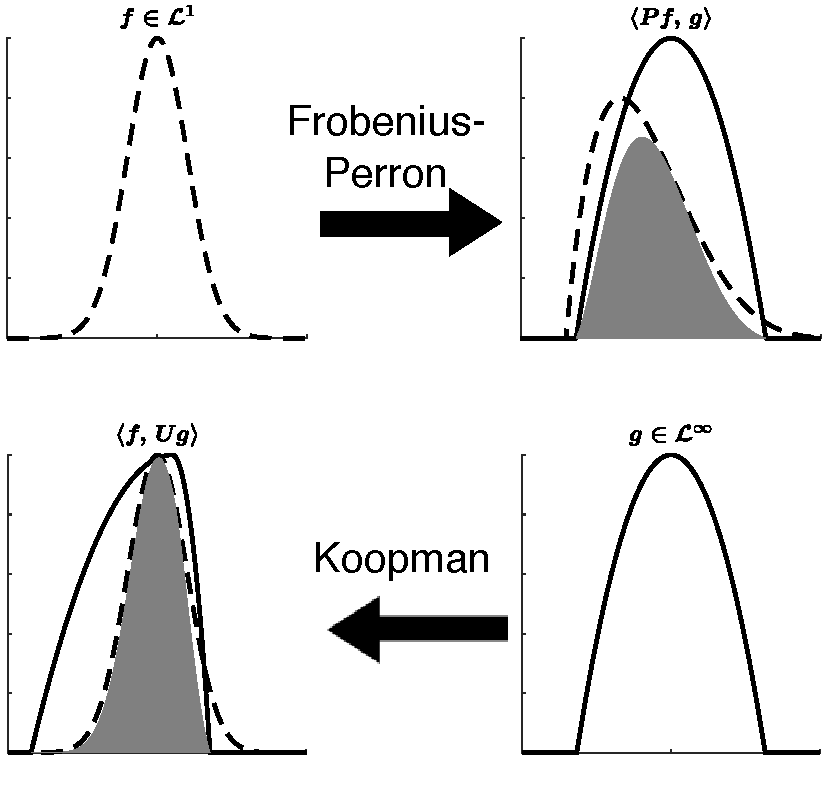
\includegraphics[width=0.5\linewidth]{img/content/chapter3/koopman_exp.pdf}
        \caption{Diagrama explicativo de la relación entre el operador de Koopman y Perron-Frobenius, obtenido de \cite{Gerlach2020TheSystems}, a su vez adaptado de \cite{Leonard2019ProbabilisticAirdrop}.}
        \label{fig:koopman_exp}
    \end{figure}
\end{obs}
Notar que, una vez realizado el \textit{embedding} a dimensión infinita de las distribuciones de probabilidad del problema, es necesario regresar al espacio de dimensión original. Por ello, se introduce un nuevo operador de Koopman que actuará como un operador de \textit{lifting back}.

Sea $\Tilde{k}_\X: \X \times \X \to \R$ el \textit{kernel} definido a partir del producto interno, con lo cual su \textit{feature map} canónico $\phi : \X \to \R^n$ está dado por la función identidad. Esto es:
\begin{equation*}
    \Tilde{k}_\X (x, y) = x^\top y, \quad \phi (x) = x.
\end{equation*}
Entonces, el operador de covarianza cruzada asociado a $X$ y a los \textit{embeddings} entre $\H_\X$ y $\R^n$, este último considerado como el RKHS asociado a $\Tilde{k}_\X$, $C_{X|X} : \H_\X \to \R^n$, debe satisfacer
\begin{equation*}
    C_{X|X} \Phi_\X (\mathbf{x}) = \mathbb{E} [\phi (X) | X = \mathbf{x}] = \mathbb{E}[ X | X = \mathbf{x}] = \mathbf{x}.
\end{equation*}

De este modo, en virtud del teorema \ref{teo:cov_koop_equiv}, se concluye que existe un operador de Koopman $\B : \R^n \to \H_\X$ tal que $C_{X|X} = \B^*$, al cual denominaremos operador de \textit{lifting back}. Este operador permitirá regresar al espacio original desde un espacio de dimensión mayor.

\begin{figure}[h!]
    \centering
    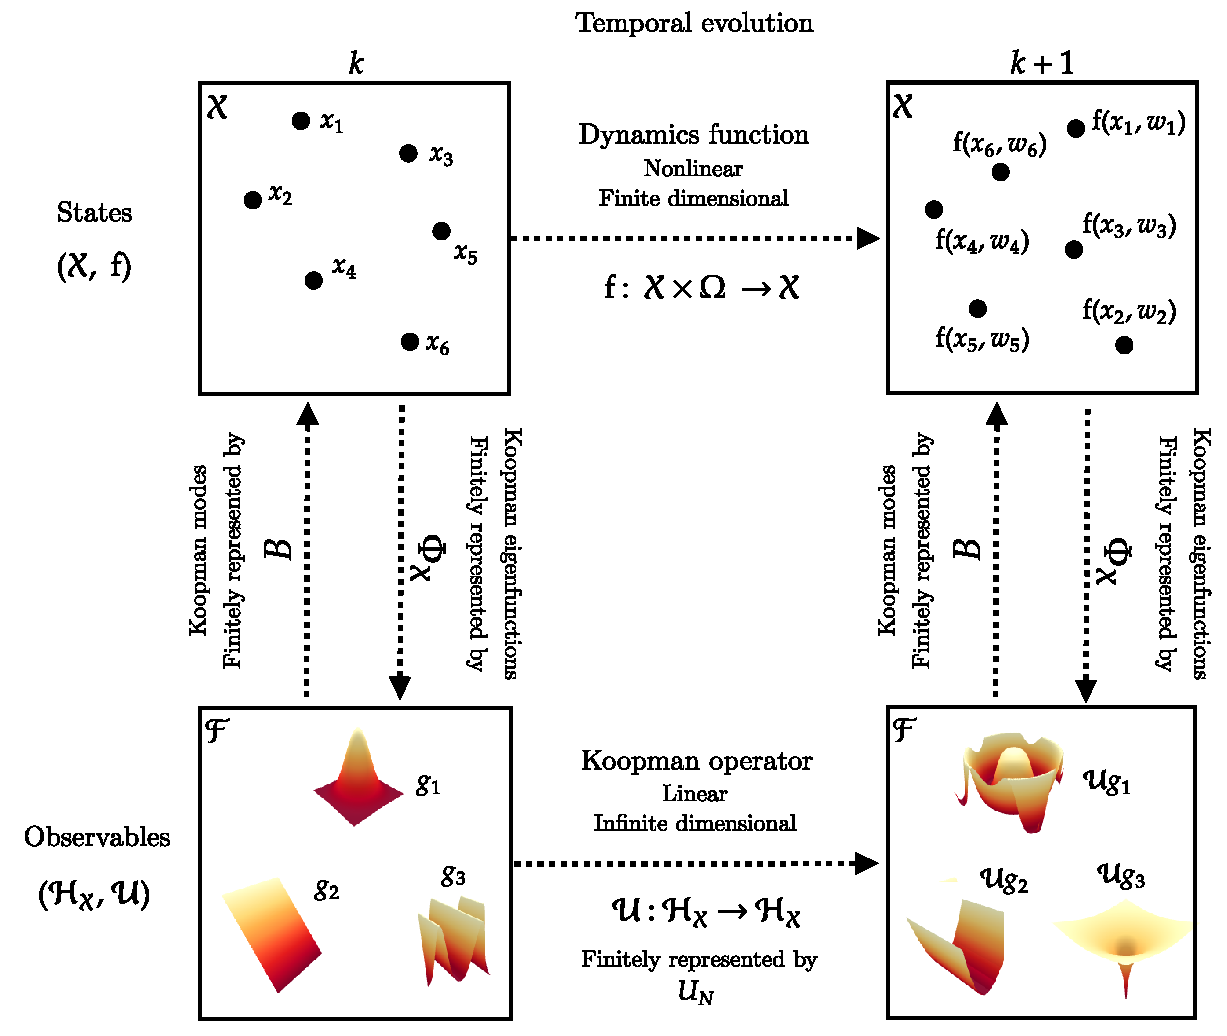
\includegraphics[width=0.8\linewidth]{img/content/chapter3/KoopDiag.pdf}
    \caption{Diagrama explicativo de las transiciones que trata de representar el operador de Koopman. Elaboración propia inspirada en la versión original en \cite{Williams2015ADecomposition}.}
    \label{fig:KoopDiag}
\end{figure}

\section{Aproximación de operadores de Koopman}

En esta sección se describe el proceso de aproximación de los operadores de Koopman relacionados con la dinámica, observación y reconstrucción. Para ello, se consideran \( N \) puntos, representados como \( \{ x_i \}_{i=1}^N \sim \mu_\X^N \), y conjuntos de puntos adicionales \( \{ x^+_i \}_{i=1}^N \) y \( \{ y_i \}_{i=1}^N \), generados bajo las siguientes distribuciones:
\begin{equation*}
    x^+_i \sim \rho_f (x_i, \cdot), \quad y_i \sim \rho_g (x_i, \cdot), \quad i = 1, \dots, N.
\end{equation*}
Se define el espacio:
\begin{equation*}
    \H_{\X, N} = \text{span} \{\Phi_\X (x_i) : i = 1, \dots, N \},
\end{equation*}
cuya base canónica está dada por \( \{\Phi_\X (x_i) : i = 1, \dots, N \} \).

Se introducen las siguientes matrices:
\begin{equation*}
    \mathbf{X} = (x_{1} | \dots | x_N), \quad \mathbf{X}^+ = (x_{1}^+ | \dots | x_N^+), \quad \mathbf{Y} = (y_1 | \dots | y_N),
\end{equation*}
\begin{equation*}
    \Phi_N (\mathbf{X}) = (k_\X(x_i, x_j))_{i,j = 1}^N, \quad \Phi_N (\mathbf{X}^+) = (k_\X(x_i, x^+_j))_{i,j = 1}^N.
\end{equation*}
Con base en estas definiciones, se introducen los operadores:
\begin{equation*}
    C_{X}^N : \H_{\X, N} \to \H_{\X, N}, \quad C_{XX^+}^N : \H_{\X, N} \to \H_{\X, N}, \quad 
\end{equation*}
\begin{equation*}
    C_{XY}^N : \R^p \to \H_{\X, N}, \quad C_{XX}^N : \R^n \to \H_{\X, N}.
\end{equation*}
definidos como
\[
C_X^N = \frac{1}{N} \sum_{j=1}^N \Phi_\X (x_j) \otimes \Phi_\X (x_j), \quad C_{XX^+}^N = \frac{1}{N} \sum_{j=1}^N \Phi_\X (x_j) \otimes \Phi_\X (x_j^+)
\]
\[
C_{XY}^N = \frac{1}{N} \sum_{j=1}^N \Phi_\X (x_j) \otimes \Phi_\Y (y_j), \quad C_{XX}^N = \frac{1}{N} \sum_{j=1}^N \Phi_\X (x_j) \otimes \phi (x_j)
\]
Entonces las acciones de estos operadores viene dada por
\begin{equation*}
    C_{X}^N \Phi_\X (x_i) = \frac{1}{N} \sum_{j = 1}^N k_\X(x_i, x_j) \Phi_\X (x_j), \quad C_{XX^+}^N \Phi_\X (x_i) = \frac{1}{N} \sum_{j = 1}^N k_\X(x_i, x_j^+) \Phi_\X (x_j),
\end{equation*}
\begin{equation*}
        C_{XY}^N \Phi_\Y (y_i) = \frac{1}{N} \sum_{j = 1}^N k_\Y (y_i, y_j) \Phi_\X (x_j), \quad C_{XX}^N \phi (x_i) = \frac{1}{N} \sum_{j = 1}^N \langle x_i, x_j \rangle \Phi_\X (x_j).
\end{equation*}
Estos operadores están representados mediante las matrices \( \Phi_N (\mathbf{X}) \), \( \Phi_N (\mathbf{X}^+) \), \( \mathbf{Y} \) y \( \mathbf{X} \), respectivamente. A continuación, se definen los operadores:
\begin{equation*}
    \U_N : \H_{\X, N} \to \H_{\X, N}, \quad \G_N : \R^p \to \H_{\X, N}, \quad \B_N : \R^n \to \H_{\X, N},
\end{equation*}
los cuales están representados por las siguientes matrices:
\begin{equation*}
    \mathbf{U}_N = (\Phi_N (\mathbf{X}))^{-1} \Phi_N (\mathbf{X}^+)^\top,
\end{equation*}
\begin{equation*}
    \mathbf{G}_N = (\Phi_N (\mathbf{X}))^{-1} \mathbf{Y}^\top,
\end{equation*}
\begin{equation*}
    \mathbf{B}_N = (\Phi_N (\mathbf{X}))^{-1} \mathbf{X}^\top.
\end{equation*}
es decir,
\begin{equation*}
    \U_N = (C_X^N)^{-1} C_{XX^+}^N,
\end{equation*}
\begin{equation*}
    \G_N = (C_X^N)^{-1} C_{XY}^N,
\end{equation*}
\begin{equation*}
    \B_N = (C_X^N)^{-1} C_{XX}^N.
\end{equation*}
El algoritmo \ref{alg:kEDMD} se deja el detalle para poder aplicar \textit{kernel} Extended Dynamic Mode Decomposition en el ámbito computacional.

\begin{algorithm}
\caption{kEDMD($\mu_\X$, $\rho_f$, $\rho_g$, $k$, $N$)}\label{alg:kEDMD}
\begin{algorithmic}[1]
\State \textbf{Entrada:} $\mu_\X$ medida de probabilidad asociada al estado, $\rho_f$ medida de probabilidad asociada a la dinámica, $\rho_g$ medida de probabilidad asociada a la observación, $\mathbf{k}: \X \times \X \to \R$ un \textit{kernel} semidefinido positivo, $N$ dimensión de aproximación de Koopman.
\State \textbf{Salida:} $\mathbf{U}_N \in \R^{N \times N}$ aproximación del operador de Koopman, $\mathbf{\Phi}_N: \X \to \R^{N}$ función de \textit{lifting forward}, $\mathbf{G}_N \in \R^{p \times N}$ matriz de linealización de la observación y $\mathbf{B}_N \in \R^{n \times N}$ matriz de \textit{lifting back}.
\State $x \sim \mu_\X, \, i = 1, \dots, N$ \Comment{$N$ muestras independientes \textit{sampleadas} desde $\mu_\X$}
\State $x_i^+ \gets \rho_f(x_i, \cdot), \, i = 1, \dots, N$ \Comment{$N$ muestras de la dinámica}
\State $y_i \gets \rho_g(x_i, \cdot), \, i = 1, \dots, N$ \Comment{$N$ muestras de la observación}
\State $\Phi_N (\cdot) \gets k(\mathbf{X}, \cdot)$
\Comment{Función de \textit{lift forward}}
\State $\Phi_N (\mathbf{X}) \gets (\mathbf{k}(x_i, x_j))_{i,j=1}^{N}$
\State $\Phi_N (\mathbf{X}^+) \gets (\mathbf{k}(x_i, x_j^+))_{i,j=1}^{N}$
\State $\mathbf{U}_N \gets \Phi_\X (\mathbf{X})^{-1}\Phi_\X (\mathbf{X}^+)^T$
\Comment{Aproximación del operador de Koopman}
\State $\mathbf{G}_N \gets \Phi_\X (\mathbf{X})^{-1} \mathbf{Y}^T$
\Comment{Aproximación del operador de observación}
\State $\mathbf{B}_N \gets \Phi_\X (\mathbf{X})^{-1} \mathbf{X}^T$
\Comment{Matriz de \textit{lift back}}
\end{algorithmic}
\end{algorithm}

Por otra parte, se definen las siguientes normas asociadas al \textit{kernel} \( k_\X \):
\begin{equation*}
    \| k_\X \|_1 = \int_\X k_\X (x,x) d \mu_\X (x), \quad \| k_\X \|_\infty = \sup_{x \in \X} k_\X (x,x),
\end{equation*}
las cuales son finitas en el caso del \textit{kernel} de Matérn. En lo que sigue se probará una cota de error para kEDMD. Para ello primero es necesario ver que algunos de los operadores se pueden extender a $\H_\X$.

\begin{prop}
    Los operadores $C_X^N$ y $C_{XX^+}^N$ se pueden extender como operadores de $\H_\X$ en $ \H_{\X, N}$ de manera continua.
\end{prop}

\begin{proof}
    Sea $\psi \in \H_\X$ y $\varepsilon > 0$ luego por Moore-Aronszajn existen $\{ \Tilde{x}_j \}_{j=1}^m$ tales que
    \[
    \psi_m = \sum_{j=1}^m \alpha_j \Phi_\X (\Tilde{x}_j)
    \]
    cumple $\psi_m \in \H_{\X, m} := \text{span}(\{ \Phi_\X (\Tilde{x}_j), \, j=1,\dots,m \})$ y $\| \psi - \psi_m \| \leq \varepsilon$. Primero se extienden los operadores a espacios finitamente generados como $\H_{\X, m}$, para ello se hace uso de la acción de estos sobre $\Phi_\X (x_i)$, quedando
    \[
    C_X \psi_m =
    \frac{1}{N} \sum_{i=1}^m \alpha_i \sum_{j = 1}^N k_\X(\Tilde{x}_i, x_j) \Phi_\X (x_j), \quad C_{XX^+} \psi_m =
    \frac{1}{N} \sum_{i=1}^m \alpha_i \sum_{j = 1}^N k_\X(\Tilde{x}_i, x_j^+) \Phi_\X (x_j).
    \]
    Entonces se extienden a $\H_\X$ como
    \[
    C_X \psi = \lim_{m \to \infty} C_X \psi_m, \quad C_{XX^+} \psi = \lim_{m \to \infty} C_{XX^+} \psi_m,
    \]
    de forma que
    \[
    C_X \psi =
    \frac{1}{N} \sum_{i \geq 1} \alpha_i \sum_{j = 1}^N k_\X(\Tilde{x}_i, x_j) \Phi_\X (x_j), \quad C_{XX^+} \psi =
    \frac{1}{N} \sum_{i \geq 1} \alpha_i \sum_{j = 1}^N k_\X(\Tilde{x}_i, x_j^+) \Phi_\X (x_j).
    \]
    Con ello basta ver que está definido de manera continua
    \[
    \begin{aligned}
        \| C_X \psi \|^2 & \leq \frac{1}{N^2} \sum_{i \geq 1} \sum_{j=1}^N \alpha_i^2 k(\Tilde{x}_i, x_j)^2 \| \Phi_\X (x_j) \|^2 \\
        & \leq \frac{\| k \|_\infty^2}{N^2} \| \alpha \|_{\ell^2} \sum_{j=1}^N k(x_j, x_j) \\
        & \leq \frac{\| k \|_\infty^2}{N^2} \| \psi \|_{\H_\X} \sum_{j=1}^N k(x_j, x_j). \\
    \end{aligned}
    \]
    Análogamente
    \[
    \| C_{XX^+} \psi \| \leq \frac{\| k \|_\infty^2}{N^2} \| \psi \|_{\H_\X} \sum_{j=1}^N k(x_j, x_j),
    \]
    con lo que los operadores se extienden de manera continua.
\end{proof}

Una desigualdad que será clave es la desigualdad de Hoeffding, que es corolario de un teorema asociado a martingalas, probado por Pinelis en 1994.

\begin{teo}[\cite{Pinelis1994OptimumSpaces} Teorema 3.5]
Sea $(S_k)_{k \in \mathbb{N}}$ una sucesión de martingalas con valores en un espacio de Hilbert real separable $H$ tal que 
\[
\sum_{k=1}^\infty \operatorname{ess\,sup} \|S_k - S_{k-1}\|_H^2 \leq C^2
\]
para alguna constante $C^2 > 0$. Entonces, para todo $\varepsilon > 0$, se tiene
\[
\mathbb{P} \left( \sup_{k \in \mathbb{N}} \|S_k\|_H \geq \varepsilon \right) \leq 2 \exp \left( -\frac{\varepsilon^2}{2C^2} \right).
\]
\end{teo}

\begin{cor}[Desigualdad de Hoeffding en espacios de Hilbert]
Sean $\xi_1, \dots, \xi_n$ variables aleatorias independientes en un espacio de Hilbert separable $H$ tales que $\mathbb{P}$-c.t.p. $\|\xi_i\|_H \leq M$ y $\mathbb{E}[\xi_i] = 0$ para todo $1 \leq i \leq n$. Entonces, para todo $\varepsilon > 0$, se tiene
\[
\mathbb{P} \left( \left\| \frac{1}{n} \sum_{i=1}^n \xi_i \right\|_H \geq \varepsilon \right) \leq 2 \exp \left( -\frac{n\varepsilon^2}{2M^2} \right).
\]
\end{cor}

Ahora un lema probado por Philipp et al. \cite{Philipp2024ErrorOperator} será relevante para las proposiciones venideras.

\begin{lema}
    Las siguientes son equivalentes
    \begin{enumerate}
        \item $\U \H_\X \subseteq \H_\X$.
        \item $\U \in \mathcal{L}(\H_\X, \H_\X)$.
        \item $\text{Ran}(C_{XX^+}) \subseteq \text{Ran}(C_X).$
    \end{enumerate}
\end{lema}

Primero se procede de la misma forma en que lo hicieron Philipp et al. \cite{Philipp2024ErrorOperator}, utilizando la desigualdad de Hoeffding para obtener una cota de probabilidad para la aproximación del operador.

\begin{prop}
    Sean $\varepsilon > 0$ y $N \in \N$, luego con probabilidad $(1-\delta)^4$ se tiene que
    \[
    \| C_{X} - C_{X}^N \|, \, \| C_{XX^+} - C_{XX^+}^N \|, \, \| C_{XY} - C_{XY}^N \|, \, \| C_{XX} - C_{XX}^N \| \leq \varepsilon.
    \]
    con 
    \[
    \delta = 2 \text{exp} \left ( 
    -\frac{N \varepsilon^2}{8 \| k\|_\infty} \right )
    \]
\end{prop}

\begin{proof}
        Primero notar que para $\psi \in \H_\X$ se tiene
    \[
    \| (\Phi_\X (x_j) \otimes \Phi_\X (x_j))\psi \|^2 = \| \psi(x_j) \Phi_\X (x_j) \|^2 \leq \| \psi \|_\infty^2 k(x_j, x_j) \leq \| k \|_\infty \| \psi \|_{\H_\X}.
    \]
    Se concluye que
    \[ \| \Phi_\X (x_j) \otimes \Phi_\X (x_j) \| \leq  \sqrt{\| k \|_\infty.} \] 
    Análogamente,
    \[
    \| \Phi_\X (x_j) \otimes \Phi_\X (x_j^+) \| \leq \sqrt{\| k \|_\infty},
    \]
     \[
    \| \Phi_\X (x_j) \otimes \Phi_\Y (y_j) \| \leq \sqrt{\| k \|_\infty},
    \]
     \[
    \| \Phi_\X (x_j) \otimes \phi (x_j) \| \leq \sqrt{\| k \|_\infty}.
    \]
    Por lo que
    \[ \| \E[ \Phi_\X (x_j) \otimes \Phi_\X (x_j)] \| \leq  \E[ \| \Phi_\X (x_j) \otimes \Phi_\X (x_j) \| ] \leq \sqrt{\| k \|_\infty}, \] 
    \[
    \| \E[ \Phi_\X (x_j) \otimes \Phi_\X (x_j^+)] \| \leq \E[ \| \Phi_\X (x_j) \otimes \Phi_\X (x_j^+)\|]  \leq \sqrt{\| k \|_\infty},
    \]
     \[
    \| \E [\Phi_\X (x_j) \otimes \Phi_\Y (y_j)] \| \leq \E [\| \Phi_\X (x_j) \otimes \Phi_\Y (y_j) \|]  \leq \sqrt{\| k \|_\infty},
    \]
     \[ \| \E[ \Phi_\X (x_j) \otimes \phi (x_j)] \| \leq  \E[ \| \Phi_\X (x_j) \otimes \phi (x_j) \| ] \leq \sqrt{\| k \|_\infty}. \] 
     Obteniendo que
     \[
     \| \Phi_\X (x_j) \otimes \Phi_\X (x_j) - C_X \| \leq \| \Phi_\X (x_j) \otimes \Phi_\X (x_j) \| + \| C_X \| \leq 2 \sqrt{\| k \|_\infty},
     \]
     \[
     \| \Phi_\X (x_j) \otimes \Phi_\X (x_j^+) - C_{XX^+} \| \leq \| \Phi_\X (x_j) \otimes \Phi_\X (x_j^+) \| + \| C_{XX^+} \| \leq 2 \sqrt{\| k \|_\infty},
     \]
     \[
     \| \Phi_\X (x_j) \otimes \Phi_\Y (y_j) - C_{XY} \| \leq \| \Phi_\X (x_j) \otimes \Phi_\Y (y_j) \| + \| C_{XY} \| \leq 2 \sqrt{\| k \|_\infty},
     \]
    \[
     \| \Phi_\X (x_j) \otimes \phi (x_j) - C_{XX} \| \leq \| \Phi_\X (x_j) \otimes \phi (x_j) \| + \| C_{XX} \| \leq 2 \sqrt{\| k \|_\infty}.
     \]

     Sea $\varepsilon > 0$ y $N \in \N$, se denota
     \[
     \delta = 2 \text{exp} \left ( - \frac{N \varepsilon^2}{8 \| k \|_\infty} \right )
     \]
     luego por desigualdad de Hoeffding se tiene que
    \[
    \P ( \| C_{X} - C_{X}^N \| > \varepsilon ) \leq \delta,
    \]
    \[
    \P ( \| C_{XX^+} - C_{XX^+}^N \| > \varepsilon ) \leq \delta,
    \]
    \[
    \P ( \| C_{XY} - C_{XY}^N \| > \varepsilon ) \leq \delta,
    \]
    \[
    \P ( \| C_{XX} - C_{XX}^N \| > \varepsilon ) \leq \delta.
    \]
    Entonces
    \[
    \P ( \| C_{X} - C_{X}^N \| \leq \varepsilon ) \geq 1-\delta,
    \]
    \[
    \P ( \| C_{XX^+} - C_{XX^+}^N \| \leq \varepsilon ) \geq 1-\delta,
    \]
    \[
    \P ( \| C_{XY} - C_{XY}^N \| \leq \varepsilon ) \geq 1-\delta,
    \]
    \[
    \P ( \| C_{XX} - C_{XX}^N \| \leq \varepsilon ) \geq 1-\delta.
    \]
    Con lo que con probabilidad al menos $(1-\delta)^4$ se tiene que
    \[
    \| C_{X} - C_{X}^N \|, \, \| C_{XX^+} - C_{XX^+}^N \|, \, \| C_{XY} - C_{XY}^N \|, \, \| C_{XX} - C_{XX}^N \| \leq \varepsilon.
    \]
\end{proof}

Algo que se usará de manera recurrente es la inyectividad de $C_X$, específicamente la cota inferior que se tiene cuando operadores lineales son inyectivos.

\begin{lema}[\cite{Christmann2008SupportMachines}]
    $C_X$ es inyectivo; de forma equivalente, existe una constante $c_1 > 0$ tal que
    \[
    \| C_X \psi \| \geq c_1 \| \psi \|, \quad \forall \psi \in \H_\X.
    \]
    A la constante $c_1$ se le denotará la constante de inyectividad de $C_X$.
\end{lema}


A continuación se presenta la cota para aproximación de los operadores de Koopman que es un aporte original de este trabajo, que busca dar una cota de error de orden $O(N^{-1/2})$, con el objetivo de competir con otras cotas existentes en la literatura para filtros no lineales.

\begin{teo}[Cota para kEDMD]
\label{teo:error_koop_sqrt_N_def}
Sean $\delta \in (0, 1)$ y $N \in \N$ tales que
\[
\delta > 2 \text{exp} \left ( -\frac{Nc_1^2}{8\|k\|_\infty}\right )
\]
con $c_1$ la constante de inyectividad de $C_X$. Luego si $\U \H_\X \subset \H_\X, \, \G (\R^p)^* \subset \H_\X, \, \B (\R^n)^* \subset \H_\X$, se tiene con probabilidad $(1-\delta)^4$ que 
 \begin{equation}
    \| \U - \U_N \|_{\H_{\X} \to \H_{\X}} \leq C_\delta N^{-1/2},
    \label{eq:kEDMD_bound}
\end{equation}
\begin{equation*}
\| \G - \G_N \|_{\R^p \to \H_{\X}} \leq C_\delta N^{-1/2},
\end{equation*}
\begin{equation*}
\| \B - \B_N \|_{\R^n \to \H_{\X}} \leq C_\delta N^{-1/2},
\end{equation*}
donde 
\[
C_\delta = \left ( \frac{2}{c_1} + \frac{\sqrt{\| k \|_{\infty}}}{c_1^2}
  \right )\sqrt{8 \| k \|_\infty \ln \left ( \frac{2}{\delta}\right ) }.
\]
\end{teo}

\begin{proof}
    Sea $\psi \in \H_\X$, luego
    \[
    \begin{aligned}
        \| \U \psi - \U_N \psi \| &= \| C_X^{-1} C_{XX^+} \psi - \left (C_X^N \right )^{-1} C_{XX^+}^N \psi \| \\
        & \leq \| C_X^{-1} C_{XX^+} \psi - C_X^{-1} C_{XX^+}^N \psi \| + \| C_X^{-1} C_{XX^+}^N \psi - \left (C_X^N \right )^{-1} C_{XX^+}^N \psi \|.
    \end{aligned}
    \]
    Viendo el primer término:
    \[ \| C_X^{-1} C_{XX^+} \psi - C_X^{-1} C_{XX^+}^N \psi \|, \]
    sean
    \[ \Tilde{\psi} = C_{XX^+} \psi, \quad  \Tilde{\psi}_N = C_{XX^+}^N \psi, \]
    con lo que 
    \[ \| C_X^{-1} C_{XX^+} \psi - C_X^{-1} C_{XX^+}^N \psi \| = \| C_X^{-1} \Tilde{\psi} - C_X^{-1} \Tilde{\psi}_N \|, \]
    luego sean $\hat{\psi}$ y $\hat{\psi}_N$ tales que 
    \[ C_X \hat{\psi} = \Tilde{\psi}, \quad C_X \hat{\psi}_N = \Tilde{\psi}_N \]
    que existen dado que $\text{Ran}(C_{XX^+}) \subseteq \text{Ran}(C_X)$.

    Luego, 
    \[
    \| C_X^{-1} C_{XX^+} \psi - C_X^{-1} C_{XX^+}^N \psi \| = \|\hat{\psi} - \hat{\psi}_N \|.
    \]
    Por inyectividad de $C_X$, existe $c_1$ tal que
    \[
    c_1 \| \hat{\psi} - \hat{\psi}_N  \| \leq \| C_X \hat{\psi} - C_X \hat{\psi}_N \| = \| \Tilde{\psi} - \Tilde{\psi}_N \| \leq \| C_{XX^+} - C_{XX^+}^N \| \| \psi \| \leq \varepsilon \| \psi \|,
    \]
    de lo que se obtiene que 
    \[
    \| C_X^{-1} C_{XX^+} \psi - C_X^{-1} C_{XX^+}^N \psi \| \leq \frac{\varepsilon}{c_1} \| \psi \|.
    \]

    Ahora para el término
    \[
    \| C_X^{-1} C_{XX^+}^N \psi - \left (C_X^N \right )^{-1} C_{XX^+}^N \psi \|,
    \]
    se denota
    \[
    \Tilde{\psi}_N = C_{XX^+}^N \psi,
    \]
    con lo que
    \[
    \| C_X^{-1} C_{XX^+}^N \psi - \left (C_X^N \right )^{-1} C_{XX^+}^N \psi \| = \| C_X^{-1} \Tilde{\psi}_N - \left (C_X^N \right )^{-1} \Tilde{\psi}_N \|.
    \]

    Notar que,
    \[
    \Tilde{\psi}_N \in 
   \H_{\X, N} = \text{Ran}(C_{X}^N) = \text{Ran}(C_{XX^+}^N) \subseteq \text{Ran}(C_{XX^+}) \subseteq \text{Ran}(C_X)
    \]
    por lo que $\Tilde{\psi}_N \in \text{Ran}(C_{X}^N)$ y $\Tilde{\psi}_N \in \text{Ran}(C_{X})$. Así, existen $\hat{\psi}_N$, $\hat{\psi}$ tal que
    \[
    C_X^N \hat{\psi}_N = \Tilde{\psi}_N, \quad C_X \hat{\psi} = \Tilde{\psi}_N,
    \]
    con lo que,
    \[
    \| C_X^{-1} C_{XX^+}^N \psi - \left (C_X^N \right )^{-1} C_{XX^+}^N \psi \| = \| \hat{\psi}_N - \hat{\psi}\|
    \]
    luego, $C_X^N \hat{\psi}_N = C_X \hat{\psi}$ y así
    \[
    C_X \hat{\psi} - C_X \hat{\psi}_N = C_X^N \hat{\psi}_N - C_X \hat{\psi}.
    \]
    Por inyectividad de $C_X$, se tiene que
    \[
    c_1 \| \hat{\psi} - \hat{\psi}_N \| \leq  \| C_X \hat{\psi} - C_X \hat{\psi}_N \| \leq \| C_X^N \hat{\psi}_N - C_X \hat{\psi}_N \| \leq \| C_X^N - C_X\| \| \hat{\psi}_N \| \leq \varepsilon \| \hat{\psi}_N \|,
    \]
    es decir,
    \[
    \| \hat{\psi} - \hat{\psi}_N \| \leq \frac{\varepsilon}{c_1} \| \hat{\psi}_N \|.
    \]
    
    Por otro lado, 
    \[
    C_X^N \hat{\psi}_N = C_X \hat{\psi}_N + (C_X^N - C_X) \hat{\psi}_N,
    \]
    y con ello
    \[
    -C_X \hat{\psi}_N = -C_X^N \hat{\psi}_N + (C_X^N - C_X) \hat{\psi}_N,
    \]
    con lo que
    \[
    \| C_X \hat{\psi}_N \| \leq \| C_X^N \hat{\psi}_N \| + \| (C_X^N - C_X) \hat{\psi}_N \| \leq \| C_X^N - C_X \| \| \hat{\psi}_N \| \leq \varepsilon \| \hat{\psi}_N \|,
    \]
    de lo que se sigue que
    \[
    \| C_X \hat{\psi}_N \| - \varepsilon \| \hat{\psi}_N \| \leq \| C_X^N \hat{\psi}_N \|.
    \]
    Por inyectividad de $C_X$ se tiene que
    \[
    c_1 \| \hat{\psi}_N \| - \varepsilon \| \hat{\psi}_N \| \leq \| C_X \hat{\psi}_N \| - \varepsilon \| \hat{\psi}_N \| \leq \| C_X^N \hat{\psi}_N \|.
    \]
    Recordando que $C_X^N \hat{\psi}_N =  \Tilde{\psi}_N$ y $\Tilde{\psi}_N = C_{XX^+}^N \psi$, se obtiene
    \[
    (c_1 - \varepsilon) \| \hat{\psi}_N \| \leq \| C_X^N \hat{\psi}_N \| = \| \Tilde{\psi}_N \| = \| C_{XX^+}^N \psi \| \leq \| C_{XX^+}^N \| \| \psi \|.
    \]
    Si $\varepsilon < c_1$, se obtiene que
    \[
    \| \hat{\psi}_N \| \leq \frac{1}{c_1 - \varepsilon}
    (\| C_{XX^+} \| + \| C_{XX^+} - C_{XX^+} \| ) \| \psi \|.
    \]

    Con todo esto
    \[
    \begin{aligned}
        \| \hat{\psi} - \hat{\psi}_N \| & \leq \frac{\varepsilon}{c_1(c_1 - \varepsilon)}
    (\| C_{XX^+} \| + \| C_{XX^+} - C_{XX^+} \| ) \| \psi \| \\
    & \leq \frac{\varepsilon}{c_1^2}
    (\| C_{XX^+} \| + \varepsilon ) \| \psi \| \\
    & \leq \frac{\varepsilon}{c_1^2}
    (\| C_{XX^+} \| + c_1 ) \| \psi \|.
    \end{aligned}
    \]
    Con lo que
    \[
    \| C_X^{-1} C_{XX^+}^N \psi - \left (C_X^N \right )^{-1} C_{XX^+}^N \psi \| \leq \frac{\varepsilon}{c_1^2}
    (\| C_{XX^+} \| + c_1 ) \| \psi \|,
    \]
    y así
    \[
    \| \U \psi - \U_N \psi \| \leq \frac{\varepsilon}{c_1} \| \psi \| + \frac{\varepsilon}{c_1^2}
    (\| C_{XX^+} \| + c_1 ) \| \psi \|,
    \]
    de lo que se concluye que
    \[
    \| \U - \U_N \| \leq \left ( \frac{1}{c_1} + \frac{1}{c_1^2}
    (\| C_{XX^+} \| + c_1 ) \right ) \varepsilon \leq \left ( \frac{1}{c_1} + \frac{1}{c_1^2}
    (\sqrt{\| k \|_{\infty}} + c_1 ) \right ) \varepsilon.
    \]

    Si
    \[
    \delta > 2\text{exp} \left ( - \frac{N c_1^2}{8 \| k \|_\infty} \right ),
    \]
    entonces
    \[
    8 \| k \|_{\infty} \ln \left ( \frac{2}{\delta} \right ) < N c_1^2,
    \]
    con lo que
    \[
    \sqrt{8 \| k \|_{\infty} \ln \left ( \frac{2}{\delta} \right )} < N^{1/2} c_1,
    \]
    así $C_\delta N^{-1/2} < c_1$. Entonces, llamando
    \[
    \varepsilon = C_\delta N^{-1/2} < c_1
    \]
    se tiene
     \[
    \| \U - \U_N \| \leq \left ( \frac{2}{c_1} + \frac{\sqrt{\| k \|_{\infty}}}{c_1^2}
  \right )\sqrt{8 \| k \|_\infty \ln \left ( \frac{2}{\delta}\right ) } N^{-1/2}.
    \]
\end{proof}

\begin{obs}
    Sobre la constante $c_1$ no se saben muchas cosas, solo que debe estar acotada por la norma del operador $C_X$, esto ya que
    \[
    c_1 \| \psi \| \leq \| C_X \psi \| \leq \| C_X\| \| \psi \| \leq \sqrt{\| k \|_\infty} \| \psi \|, \quad \forall \psi \in \H_\X \setminus \{ 0 \},
    \]
    con lo que
    \[
    c_1 \leq \sqrt{\| k \|_\infty}.
    \]

    Esto no es tanta utilidad para las cotas probadas, pero sí lo es para determinar una probabilidad máxima de éxito dado un $N \in \N$, esto ya que

    \[
    2\text{exp} \left ( - \frac{N c_1^2}{8 \| k \|_\infty} \right ) \geq 2\text{exp} \left ( - \frac{N \| k \|_\infty}{8 \| k \|_\infty} \right ) = 2\text{exp} \left ( - \frac{N}{8} \right ).
    \]
    Con lo que la probabilidad máxima de éxito viene dada por
    \[
    \delta_{\text{max}} = \left ( 1-2\text{exp} \left ( - \frac{N}{8} \right ) \right )^4,
    \]
    que converge a $1$ cuando $N \to \infty$.

    Otro aspecto relevante es que, dado $N > 1$ siempre hay un $\delta$ que cumple la relación pedida por el teorema, que es
    \[
    \delta_{\text{adm,} N} = 2\text{exp} \left ( - \frac{(N-1) c_1^2}{8 \| k \|_\infty} \right ),
    \]
    que, aunque no sea realmente conocido en la práctica debido a que $c_1$ no es conocido, describe exactamente el decaimiento exponencial de la probabilidad de fracaso, cuando $N \to \infty$.

    Además, se puede obtener una cota inferior para la constante $C_\delta$ y estimar su crecimiento
    \[
     \Tilde{C}_\delta = \frac{3}{\sqrt{\| k \|_{\infty}}}\sqrt{8 \| k \|_\infty \ln \left ( \frac{2}{\delta}\right ) } \leq \left ( \frac{2}{c_1} + \frac{\sqrt{\| k \|_{\infty}}}{c_1^2}
  \right )\sqrt{8 \| k \|_\infty \ln \left ( \frac{2}{\delta}\right ) } \leq C_\delta 
    \]
    Como se observa en la tabla \ref{tab:ctes_cota_kEDMD}, el crecimiento de esta constante es bastante lento, propio de un crecimiento logarítmico en una raíz cuadrada, mientras que la probabilidad de éxito crece exponencialmente, todo esto considerando $\delta_{\text{adm, N}}$.
    \begin{table}[h!]
\centering
\begin{tabular}{|c|c|c|}
\hline
$N$ & $(1-\delta_{\text{adm, N}})^4 \cdot 100 \%$ & $\Tilde{C}_{\delta_{\text{adm, N}}}$ \\ \hline
10 & 6.75\% & 4.50 \\ \hline
50 & 10.37\% & 10.50 \\ \hline
100 & 68.38\% & 14.92 \\ \hline
200 & 98.42\% & 21.16 \\ \hline
300 & 99.93\% & 25.94 \\ \hline
\end{tabular}
\caption{Valores de $(1-\delta_{\text{adm, N}})^4 \cdot 100 \%$ y $C_{\delta_{\text{adm, N}}}$ para diferentes valores de $N$. Asumiendo que $\|k\|_\infty = 1$ (caso del \textit{kernel} de Matérn) y $c_1 = 0.5$.}
\label{tab:ctes_cota_kEDMD}
\end{table}
\end{obs}

Lo valioso de este resultado es que da un régimen asintótico para $N$ y $\delta$, compatibilizando el hecho de que $\delta \to 0^+$ cuando $N \to \infty$, proponiendo una alternativa al resultado de Philipp et al. que, como se verá posteriormente, tiene un peor \textit{trade-off} entre la probabilidad $\delta$ y la cantidad de puntos \textit{sampleados} $N$.

\begin{teo}[Philipp et al. \cite{Philipp2024ErrorOperator}]
    Sea un \( N \in \mathbb{N} \) arbitrario. Se supone que los primeros \( N + 1 \) valores propios \( \lambda_j \) de \( C_X \) son simples, es decir, \( \lambda_{j+1} < \lambda_j \) para todo \( j = 1, \ldots, N \). Se definen:
    \[
    \delta_N = \min_{j=1, \ldots, N} \frac{\lambda_j - \lambda_{j+1}}{2}, \quad c_N = \frac{1}{\sqrt{\lambda_N}} + \frac{N + 1}{\delta_N \lambda_N} (1 + \|k_\X\|_{1}) \|k_\X \|^{1/2}_{1}.
    \]
    Sea además \( \varepsilon \in (0, \delta_N) \) y \( \delta \in (0, 1) \) arbitrarios, y \( N \geq  \frac{8\|k\|^2_\infty \ln(2/\delta)}{\varepsilon^2} \). Si 
    \begin{equation*}
        \U \H_\X \subset \H_\X, \, \G (\R^p)^* \subset \H_\X, \, \B (\R^n)^* \subset \H_\X
    \end{equation*}
    entonces, con probabilidad al menos \( (1 - \delta)^4 \), se cumple que:
    \[
    \|\U - \U_N \|_{\H_{\X, N} \to L^2(\X; \mu_\X)} \leq \sqrt{\lambda_{N+1}} \|\U \|_{\H_{X} \to \mathcal{H_\X}} + c_N \varepsilon
    \]
    \[
    \|\G - \G_N \|_{\R^p \to L^2(\X; \mu_\X)} \leq \sqrt{\lambda_{N+1}} \|\G \|_{\R^p \to \mathcal{H_\X}} + c_N \varepsilon
    \]
    \[
    \|\B - \B_N \|_{\R^n \to L^2(\X; \mu_\X)} \leq \sqrt{\lambda_{N+1}} \|\B \|_{\R^n \to \mathcal{H_\X}} + c_N \varepsilon.
    \]
    \label{teo:error_koop}
\end{teo}

Un teorema de Santin et al. permite cuantificar el decaimiento de los valores propios del \textit{kernel} de Matérn, lo que será de utilidad para derivar una cota más explícita en base al resultado de Philipp et al. 

\begin{teo}[Santin et al. \cite{Santin2016ApproximationSpaces}]
    Si $\H_\X$ es equivalente en norma a un espacio de Sobolev $H^{\nu + n/2}$ y $\lambda_j$ son los valores propios de $C_X$ en orden descendente, luego
    \begin{equation*}
        \sqrt{\lambda_{N+1}} \leq C_\nu N^{-(\nu + n)/(2n)}
    \end{equation*}
    con $C_\nu$ alguna constante que no depende de $N$.
    \label{teo:eig_val_decay}
\end{teo}

De lo demostrado por Philipp et al. se desprende el siguiente teorema, que es el caso en donde se busca que el lado derecho de las desigualdades de los operadores sea $O(N^{-1/2})$. Esta cota presenta el problema de que, para alcanzar dicho orden de convergencia, se debe acotar mucho la probabilidad de éxito, incluso no se cumple que cuando $N \to \infty$ la probabilidad tiende a $0$. 

Es más, cuando $N \to \infty$ se tiene que el lado derecho tiende a $0$, mientras que cuando $\delta \to 0^+$, el lado izquierdo tiende a infinito. Esto hace que el régimen de la cota probada por estos autores no sea asintótica, aspecto que sí tiene la cota probada en esta tesis.

\begin{teo}
    Bajo la misma hipótesis del teorema \ref{teo:error_koop}, sea $\delta \in (0, 1)$, si $\H_\X$ es equivalente en norma a $H^{\nu + n/2}$ y
    \[
    8\|k\|^2_\infty \ln(2/\delta) \leq \frac{1}{2} (N+1)^{-5/2},
    \]
    con probabilidad al menos $(1 - \delta)^4$ se tiene que:
    \begin{equation*}
        \| \U - \U_N \|_{\H_{\X, N} \to L^2(\X; \mu_\X)} \leq C N^{-1/2},
    \end{equation*}
    \begin{equation*}
    \| \G - \G_N \|_{\R^p \to L^2(\X; \mu_\X)} \leq C N^{-1/2},
    \end{equation*}
    \begin{equation*}
    \| \B - \B_N \|_{\R^n \to L^2(\X; \mu_\X)} \leq C N^{-1/2},
    \end{equation*}
    con $C$ alguna constante que no depende ni de $N$ ni de $\delta$.
    \label{teo:error_koop_sqrt_N_hip}
\end{teo}

\begin{proof}
    Se verá la demostración solo para $\U$, ya que para $\G$ y $\B$ es análogo. Del teorema \ref{teo:error_koop}, bajo las hipótesis mencionadas, para $\delta \in (0, 1)$ se tiene que con probabilidad al menos $1-\delta$
    \[
    \|\U - \U_N \|_{\H_{\X, N} \to L^2(\X; \mu_\X)} \leq \sqrt{\lambda_{N+1}} \|\U \|_{\H_{X} \to \mathcal{H_\X}} + c_N \varepsilon
    \]
    con $c_N$ definido en el enunciado del teorema $\ref{teo:error_koop}$ y con 
    \begin{equation}
        N \geq \frac{8\|k\|^2_\infty \ln(2/\delta)}{\varepsilon^2}.
        \label{eq:N_bound}
    \end{equation}

    Tomando, en virtud del teorema \ref{teo:eig_val_decay}, 
    \[
    \varepsilon = \frac{\delta_N \lambda_N}{C_\nu(N+1)} N^{-1/2} \leq \frac{\delta_N}{(N+1)N^{(\nu+n)/n}} N^{-1/2} <\delta_N,
    \]
    se tiene
    \[
    c_N \varepsilon = \frac{\delta_N \sqrt{\lambda_N}}{C_\nu (N+1) N^{1/2}} + \frac{N^{-1/2}}{C_\nu} (1 + \|k_\X\|_{1}) \|k_\X \|^{1/2}_{1}.
    \]
    Y notando que 
    \[
    \delta_N = \min_{j=1, \dots, N} \frac{\lambda_j - \lambda_{j+1}}{2} \leq \min_{j=1, \dots, N} \frac{\lambda_j}{2} = \frac{\lambda_N}{2},
    \]
    y llamando
    \[
    \Tilde{c}_1 = \frac{(1 + \|k_\X\|_{1}) \|k_\X \|^{1/2}_{1}}{C_\nu}
    \]
    se tiene
    \begingroup
    \allowdisplaybreaks
    \begin{align*}
        c_N \varepsilon & \leq  \frac{\lambda_N \sqrt{\lambda_N}}{2 C_\nu (N+1) N^{1/2}} + \frac{N^{-1/2}}{C_\nu} (1 + \|k_\X\|_{1}) \|k_\X \|^{1/2}_{1} \\ 
        & \leq \frac{(N-1)^{-3(n+\nu)/(2n)}}{2 C_\nu (N+1) N^{1/2}} + \Tilde{c}_1 N^{-1/2} \\
        & \leq \frac{(N+1)^{-3(n+\nu)/(2n)}}{2 C_\nu (N+1) N^{1/2}} + \Tilde{c}_1 N^{-1/2} \\
        & \leq \frac{1}{2C_\nu} N^{-1/2} + \Tilde{c}_1 N^{-1/2}.
    \end{align*}
    \endgroup
    
    Llamando $c_2 = 1/(2C_\nu) + \Tilde{c}_1$ se obtiene que 
    \[
    \|\U - \U_N \|_{\H_{\X, N} \to L^2(\X; \mu_\X)} \leq \sqrt{\lambda_{N+1}} \|\U \|_{\H_{X} \to \mathcal{H_\X}} + c_2 N^{-1/2},
    \]
    con lo que ocupando nuevamente el teorema \ref{teo:eig_val_decay}, se obtiene
    \[
    \|\U - \U_N \|_{\H_{\X, N} \to L^2(\X; \mu_\X)} \leq C_\nu \|\U \|_{\H_{X} \to \mathcal{H_\X}} N^{-(n+\nu)/(2n)} + c_2 N^{-1/2} \leq C_\nu \|\U \|_{\H_{X} \to \mathcal{H_\X}} N^{-1/2} + c_2 N^{-1/2}.
    \]
    Y denotando $C = C_\nu \|\U \|_{\H_{X} \to \mathcal{H_\X}} + c_2$ se obtiene 
    \[
    \|\U - \U_N \|_{\H_{\X, N} \to L^2(\X; \mu_\X)} \leq C N^{-1/2},
    \]
    en donde se ha ocupado que dado que $\nu > 0$, $N^{-(n+\nu)/(2n)} \leq N^{-n/(2n)} = N^{-1/2}$.

    Ahora, notar que de \ref{eq:N_bound} se tiene
    \begingroup
    \allowdisplaybreaks
    \begin{align*}
        8\|k\|^2_\infty \ln(2/\delta) & \leq N \varepsilon^2 \\
        & = N \frac{\delta_N \lambda_N N^{-1/2}}{c_1 (N+1)} \\
        & \leq \frac{\lambda_N^2 N^{1/2}}{2c_1 (N+1)} \\
        & \leq \frac{c_1 N^{-2(\nu+n)/n} N^{1/2}}{2c_1 (N+1)} \\
        & \leq \frac{ (N+1)^{-2(\nu+n)/n} (N+1)^{1/2}}{2 (N+1)} \\
        & \leq \frac{1}{2} (N+1)^{-(2(\nu+n)/n + 1/2)}. \\
        & \leq \frac{1}{2} (N+1)^{-(2n/n + 1/2)} \\
        & = \frac{1}{2} (N+1)^{-5/2}
    \end{align*}
    \endgroup
    Con lo que se obtiene la cota que relaciona $N$ con $\delta$.
\end{proof}

El teorema anterior se fundamenta en dos hipótesis: la invarianza de Koopman y la simplicidad de los valores propios de \( C_X \). La primera hipótesis no plantea mayores inconvenientes, dado que existen numerosos sistemas donde se cumple. Por ejemplo, en el caso de ruido aditivo normal y funciones dependientes del estado que sean suficientemente suaves, dicha invarianza puede verificarse de acuerdo con la proposición \ref{cor:inv_koop}.

Sin embargo, la hipótesis sobre la simplicidad de los valores propios de \( C_X \) resulta más restrictiva. Philipp et al. no proporcionan ejemplos específicos donde esta condición se cumpla. Además, se sabe que, en ciertos casos, como en el caso de \textit{kernel} de Matérn, los valores propios de \( C_X \) están relacionados con los del operador de Laplace-Beltrami asociado al espacio de estados \( \X \) \cite{Whittle1963StochasticDimensions, Borovitskiy2020MaternManifolds}. Este hecho sugiere que existen numerosos escenarios en los cuales la simplicidad de los valores propios podría no cumplirse.

Por completitud, se deja una proposición que apunta a eliminar la hipótesis sobre los valores propios de $C_X$, aunque la cota de Philipp et al. no vaya a ser la utilizada en secciones posteriores.

\begin{prop}
    Sea $A: \H_\X \to \H_\X$ un operador compacto y autoadjunto, y sea $N \in \N$ tal que existe un valor propio $\lambda_j$, con $j < N$, cuya multiplicidad es $m > 1$. Entonces, para todo $\varepsilon \in (0, \lambda_{m+j} - \lambda_{m+j+1})$, existe un operador $B^\varepsilon: \H_\X \to \H_\X$ de rango $m$ tal que $A + B^\varepsilon$ posee los primeros $N$ valores propios simples, con las mismas funciones propias, y además $\| B^\varepsilon \| \leq C \cdot \varepsilon$, para alguna constante $C > 0$.
    \label{prop:val_prop_sim}
\end{prop}

Previo a la demostración, la intuición detrás de esta proposición es que el hecho de que haya un discreto de valores propios para un operador compacto y autoadjunto, permite acomodar valores propios con multiplicidad mayor a $1$ entre $2$ valores propios, de manera que la distancia vaya haciéndose nula, como lo explica la figura \ref{fig:simple_eig_vals}.

\begin{figure}[h!]
    \centering
    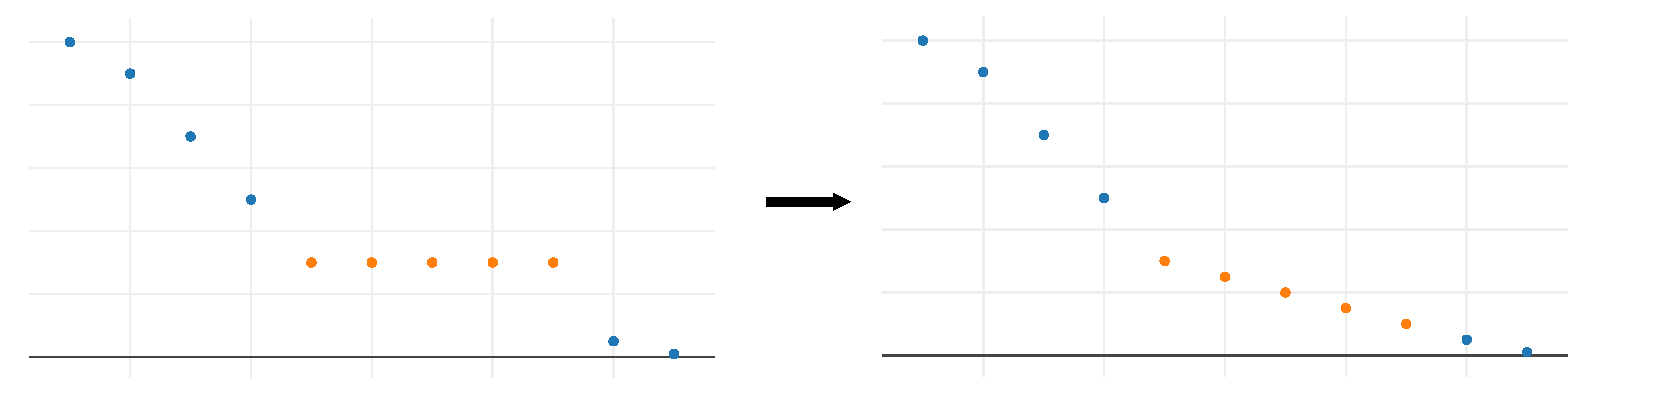
\includegraphics[width=1.0\linewidth]{img/content/chapter3/simple_eig_vals.pdf}
    \caption{Intuición de la proposición \ref{prop:val_prop_sim}. A la izquierda, en naranjo, los valores propios del operador que tienen multiplicidad mayor a $1$ y a la izquierda, en naranjo también, cómo se acomodan entre dos valores propios.}
    \label{fig:simple_eig_vals}
\end{figure}

\begin{proof}
    Dado que $\H_\X$ es un espacio de Hilbert separable y $A$ es compacto y autoadjunto, el teorema espectral \cite{Brezis2011FunctionalEquations} garantiza que $A$ posee un espectro discreto de valores propios $\{ \lambda_j \}_j$, todos positivos y decrecientes hacia $0$, con funciones propias $\{ v_j \}_j$ que constituyen una base ortonormal de $\H_\X$.

    Se definen los operadores $T_k : \H_\X \to \H_\X$ de rango $1$ como
    \[
    T_k \psi = \langle v_k, \psi \rangle v_k, \quad \psi \in \H_\X,
    \]
    los cuales son lineales y continuos. Además, satisfacen
    \[
    T_k v_\ell = \langle v_k, v_\ell \rangle v_k = \delta_{k \ell} v_k,
    \]
    donde $\delta_{k \ell}$ es la delta de Kronecker, ya que $\{ v_j \}_j$ constituye una base ortonormal.

    Sea $\varepsilon \in (0, \lambda_{m+j} - \lambda_{m+j+1})$, se define
    \[
    \varepsilon_k = \frac{\varepsilon (k-j)}{m^2 \cdot j^2}, \quad k \in \{ j, \dots , m+j \},
    \]
    que cumple $\varepsilon_k < \varepsilon < \lambda_{m+j} - \lambda_{m+j+1}$. A partir de esto, se define 
    \[
    B^\varepsilon = \sum_{k=j}^{m+j} \varepsilon_k T_k,
    \]
    el cual, al ser una suma de $m$ operadores de rango $1$ con rangos ortogonales, tiene rango $m$.

    Para \( v_\ell \) con $\ell \notin \{ j, \dots, m+j \}$, se verifica
    \[
    (C_X + B^\varepsilon) v_\ell = C_X v_\ell + B^\varepsilon v_\ell = C_X v_\ell = \lambda_\ell v_\ell.
    \]
    Es decir, $C_X + B^\varepsilon$ conserva los mismos valores propios y funciones propias de $C_X$ para $\ell \notin \{ j, \dots, m+j \}$. En cambio, para $\ell \in \{ j, \dots, m+j \}$ se tiene
    \[
    (C_X + B^\varepsilon) v_\ell = C_X v_\ell + B^\varepsilon v_\ell = \lambda_\ell v_\ell + \sum_{k=j}^{m+j} \varepsilon_k T_k v_\ell = \lambda_\ell v_\ell + \sum_{k=j}^{m+j} \varepsilon_k \delta_{k \ell} v_k = \lambda_\ell v_\ell + \varepsilon_\ell v_\ell.
    \]
    Por lo tanto,
    \[
    (C_X + B^\varepsilon)v_\ell = (\lambda_\ell + \varepsilon_\ell) v_\ell,
    \]
    lo que implica que $\Tilde{\lambda}_\ell = \lambda_\ell + \varepsilon_\ell$ es un valor propio de $C_X + B^\varepsilon$ con función propia $v_\ell$. Estos valores propios son simples ya que
    \[
    \lambda_{j-1} < \lambda_j = \lambda_j + \frac{\varepsilon (j-j)}{m^2 j^2} = \Tilde{\lambda}_j < \Tilde{\lambda}_{m+j} = \lambda_{m+j} + \frac{\varepsilon m}{m^2 j^2} < \lambda_{m+j+1}.
    \]

    En consecuencia, $C_X + B^\varepsilon$ tiene los primeros $N$ valores propios simples con las mismas funciones propias. Finalmente, para $\psi \in \H_\X$, se cumple
    \[
    \| B^\varepsilon \psi \| \leq \sum_{k=j}^{m+j} \varepsilon_k \| T_k \psi \| = \sum_{k=j}^{m+j} \varepsilon_k | \langle v_k, \psi \rangle | \| v_k \| \leq \sum_{k=j}^{m+j} \varepsilon_k \| v_k \| \| \psi \| = \sum_{k=j}^{m+j} \varepsilon_k \| \psi \|,
    \]
    con lo que
    \[
    \| B^\varepsilon \| \leq \sum_{k=j}^{m+j} \varepsilon_k  = \sum_{k=j}^{m+j} \frac{\varepsilon (k-j)}{m^2 j^2} \leq \varepsilon \sum_{k=j}^{m+j} \frac{1}{m j^2} = \frac{\varepsilon}{j^2} \leq \varepsilon \sum_{j \geq 1} \frac{1}{j^2} = C \cdot \varepsilon.
    \]

    Cabe señalar que este factor $1/j^2$ no es estrictamente necesario para una única ventana de valores propios no simples, aunque facilita la extensión de la demostración a una cantidad infinita de ventanas con dicha característica, en donde el término de la suma pasaría a ser, eventualmente, una serie lacunaria.
\end{proof}

\begin{lema}
    $C_X$ es un operador compacto y autoadjunto.
\end{lema}

\begin{proof}
    Ya se estableció previamente, en el corolario \ref{cor:CX_autoad}, que $C_X$ es autoadjunto, por lo que únicamente resta demostrar su compacidad. Sea $\{ \psi_n \}_n \subset \H_\X$ una sucesión débilmente convergente a $\psi$, es decir, para toda $\phi \in \H_\X$ y $\varepsilon > 0$, existe un $n_0 \in \N$ tal que, para $n \geq n_0$, se cumple
    \[
    \langle \psi_n - \psi, \phi \rangle \to 0.
    \]
    Se debe probar que $C_X \psi_n$ converge en norma a $C_X \psi$. Para ello, se tiene:
    \[
    \begin{aligned}
        \| C_X (\psi_n - \psi) \| & \leq \int_\X | \psi_n (x) - \psi (x) | \| \Phi_\X (x) \| d \mu_\X (x) \\
        & = \int_\X | \langle \psi_n - \psi, \Phi_\X (x) \rangle | \| \Phi_\X (x) \| d \mu_\X (x) \\
        & \leq \left ( \int_\X | \langle \psi_n - \psi, \Phi_\X (x) \rangle |^2 d \mu_\X (x) \right )^{1/2} \left ( \int_\X \| \Phi_\X (x) \|^2 d \mu_\X (x) \right )^{1/2} \\
        & = \left ( \int_\X | \langle \psi_n - \psi, \Phi_\X (x) \rangle |^2 d \mu_\X (x) \right )^{1/2} \left ( \int_\X k(x,x)^2 d \mu_\X (x) \right )^{1/2} \\
        & \to 0,
    \end{aligned}
    \]
    donde se ha aplicado la propiedad reproduciente para establecer que
    \[
    \psi_n (x) - \psi (x) = \langle \psi_n - \psi, \Phi_\X (x) \rangle,
    \]
    y la desigualdad de Hölder para separar en dos integrales.
\end{proof}

\begin{teo}
    Sea $\delta \in (0, 1)$, si $\U \H_X \subset \H_X$, $\G (\R^p)^* \subset \H_X$, $\B (\R^n)^* \subset \H_X$, $\H_\X$ es equivalente en norma a $H^{\nu + n/2}$ y 
    \[
    8\|k\|^2_\infty \ln(2/\delta) \leq \frac{1}{2} (N+1)^{-5/2},
    \]
    entonces con probabilidad al menos $(1-\delta)^4$ se tiene que
     \begin{equation*}
        \| \U - \U_N \|_{\H_{\X, N} \to L^2(\X; \mu_\X)} \leq C N^{-1/2}.
    \end{equation*}
    \begin{equation*}
    \| \G - \G_N \|_{\R^p \to L^2(\X; \mu_\X)} \leq C N^{-1/2}
    \end{equation*}
    \begin{equation*}
    \| \B - \B_N \|_{\R^n \to L^2(\X; \mu_\X)} \leq C N^{-1/2}
    \end{equation*}
    con $C$ alguna constante que no depende ni de $N$ ni de $\delta$.
\end{teo}

\begin{proof}
    Se elimina la hipótesis de la simplicidad de los valores propios de $C_X$, que es compacto y autoadjunto. Si se supone que existe un valor propio con multiplicidad mayor que $1$, entonces por la proposición \ref{prop:val_prop_sim}, se tiene que existe $B^\varepsilon$ de rango finito que cumple que $C_X + B^\varepsilon$ tiene los primeros $N+1$ valores propios simples, con las mismas funciones propias y $\| B^\varepsilon \| \leq C \varepsilon$. 

    Se define un nuevo aproximante de Koopman como
    \[
    \U^\varepsilon = (C_X + B^\varepsilon)^{-1} C_{XX^+}
    \]
    y su aproximante en dimensión finita respectivo es
    \[
    \U^\varepsilon_N = (C_X^N + B^\varepsilon)^{-1} C_{XX^+}^N
    \]
    donde $B^\varepsilon$ se deja sin cambios ya que es de rango finito. Estos operadores cumplen, para $\psi \in \H_\X$, que
    \[
    \begin{aligned}
        \| \U\psi - \U^\varepsilon\psi \| & = \| C_X^{-1} C_{XX^+} \psi - (C_X + B^\varepsilon)^{-1} C_{XX^+} \psi \| \\
        & = \| C_X^{-1} \Tilde{\psi} - (C_X + B^\varepsilon)^{-1} \Tilde{\psi} \| \\
        & = \| \hat{\psi} - \hat{\psi}_\varepsilon \|
    \end{aligned} 
    \]
    en donde
    \[
    C_{XX^+}\psi = \Tilde{\psi}, \quad C_X \hat{\psi} =  \Tilde{\psi}, \quad (C_X + B^\varepsilon)\hat{\psi}_\varepsilon = \Tilde{\psi}.
    \]
    Así
    \[
    C_X \hat{\psi} = (C_X + B^\varepsilon)\hat{\psi}_\varepsilon,
    \]
    con lo que
    \[
    C_X (\hat{\psi} - \hat{\psi}_\varepsilon) = B^\varepsilon \hat{\psi}_\varepsilon
    \]
    y así
    \[
    \|C_X (\hat{\psi} - \hat{\psi}_\varepsilon)\| = \|B^\varepsilon \hat{\psi}_\varepsilon\|.
    \]

    Gracias a la inyectividad de $C_X$, existe una constante $c_1$ tal que 
    \[
    \| \hat{\psi} - \hat{\psi}_\varepsilon \| \leq \frac{1}{c_1} \| C_X (\hat{\psi} - \hat{\psi}_\varepsilon) \| \leq \| B^\varepsilon \| \| \hat{\psi}_\varepsilon \| \leq C \cdot \varepsilon \| \hat{\psi}_\varepsilon \|. 
    \]
    Con ello notar que
    \[
    C_X \hat{\psi}_\varepsilon  = -B^\varepsilon \hat{\psi}_\varepsilon  + (B^\varepsilon + C_X)\hat{\psi}_\varepsilon
    \]
    así
    \[
    \| C_X \hat{\psi}_\varepsilon \| \leq \| B^\varepsilon \hat{\psi}_\varepsilon \| + \| (B^\varepsilon + C_X)\hat{\psi}_\varepsilon\| \leq C \cdot \varepsilon  \| \hat{\psi}_\varepsilon \| + \| (B^\varepsilon + C_X)\hat{\psi}_\varepsilon\|. 
    \]
    
    Utilizando la inyectividad de $C_X$
    \[
    c_1 \|\hat{\psi}_\varepsilon\| \leq \| C_X \hat{\psi}_\varepsilon \| \leq  C \cdot \varepsilon  \| \hat{\psi}_\varepsilon \| + \| (B^\varepsilon + C_X)\hat{\psi}_\varepsilon\|
    \]
    con ello
    \[
    (c_1 - C\varepsilon)  \|\hat{\psi}_\varepsilon\| \leq \| (B^\varepsilon + C_X)\hat{\psi}_\varepsilon\| = \| \Tilde{\psi} \|
    \]
    Tomando $\varepsilon$ tal que $c_1 - C \varepsilon > 0$ se tiene que
    \[
    \|\hat{\psi}_\varepsilon\| \leq \frac{1}{c_1 - C\varepsilon} \| \Tilde{\psi} \| = \frac{1}{c_1 - C\varepsilon} \| C_{XX^+} \psi \| \leq \frac{1}{c_1 - C\varepsilon} \| C_{XX^+} \| \| \psi \|
    \]
    Y así
    \[
     \| \U\psi - \U^\varepsilon\psi \| = \| \hat{\psi} - \hat{\psi}_\varepsilon \| \leq \frac{C \cdot \varepsilon}{c_1 - C \cdot \varepsilon} \| C_{XX^+} \| \| \psi \| \leq \frac{C \cdot \varepsilon}{c_1} \| C_{XX^+} \| \| \psi \| = c_2 \| \psi \|.
    \]

    De manera análoga, existe una constante $c_3$ tal que 
    \[
    \| \U^\varepsilon_N - \U_N \| \leq c_3 \cdot \varepsilon.
    \]
    Luego, al igual que antes se tiene
    \[
    \begin{aligned}
        \| \U - \U_N \| & \leq \| \U - \U^\varepsilon \| + \| \U^\varepsilon - \U_N^\varepsilon \| + \| \U_N^\varepsilon - \U_N \| \\
        & \leq c_2 \cdot \varepsilon + C N^{-1/2} + c_3 \cdot \varepsilon.
    \end{aligned}
    \]

   Tomando $\varepsilon = c_4 N^{-1/2}$, con $c_4 = c_1/(2C)$ que cumple
   \[
   C  \varepsilon = C c_4 N^{-1/2} \leq C c_4 = c_1/2 < c_1
   \]
   con lo que se cumple la condición $c_1 - C  \varepsilon > 0$, se tiene
   \[
   \| \U - \U_N \| \leq c_5 N^{-1/2}.
   \]
\end{proof}

\section{Resultados numéricos}

A pesar de que las cotas de error del \textit{kernel} Extended Dynamic Mode Decomposition serán útiles para la construcción de la cota de error para el filtro, también son interesantes por sí solas y se puede visualizar al aproximar distintos sistemas dinámicos y operadores de manera empírica.
Será de interés en esta sección no solo explorar cómo un sistema lineal puede aproximar otro sistema de interés mediante el \textit{sampleo} de datos, sino también el orden de decaimiento del error cometido en función del número de puntos \textit{sampleados} $N$.

\subsection{kEDMD para el caso lineal}

Un primer caso de interés es estudiar qué ocurre cuando se tiene un sistema lineal, esto es considerar un sistema de la forma
\begin{equation*}
    \mathbf{x}_{k+1} = \mathbf{A} \mathbf{x}_{k}.
\end{equation*}
Para este ejemplo se considera
\begin{equation*}
    \mathbf{A} = 
    \begin{pmatrix}
        1.01 & 0.04 & 0 \\
        0.01 & 1.02 & \alpha \\
        0 & 0.04 & 1.02
    \end{pmatrix}
\end{equation*}
en donde el parámetro $\alpha$ determinará el comportamiento del sistema dinámico en el tiempo. Se considera como distribución de probabilidad en $\X = \R^n$ una normal $N(0_{3}, 3 \cdot I_{3\times3})$, para la dinámica se considera un ruido normal $N(0_{3}, 10^{-7} \cdot I_{3\times3})$ y $\mathbf{x}_0 = (0.1, 0.1, 0.1)^T$ como condición inicial. Notar que en este ejemplo no se satisface la hipótesis de compacidad, pero el sistema con alta probabilidad se mantiene en un compacto en horizonte de tiempo finito.

Se compara la dinámica original con aquella linealizada vía Operador de Koopman \textit{sampleando} 2500 puntos del espacio de estados, utilizando \textit{kernel} de Matérn de parámetro $\nu = 1/2$ y un ancho de banda $\gamma = 10^{-3}$. Esto es, se compara con el sistema
\begin{align*}
    \mathbf{z}_{k+1} = & \mathbf{U}_N \mathbf{z}_k \\
    \hat{\mathbf{x}}_k = & \mathbf{B}_N \mathbf{z}_k \\
    \mathbf{z}_0 = & \Phi_N(\mathbf{x}_0)
\end{align*}

Se compara lo obtenido para $\alpha \in \{ -0.3, -0.1, 0.05\}$.
\begin{figure}[htbp]
    \centering
    \begin{subfigure}[b]{0.32\textwidth}
        \centering
        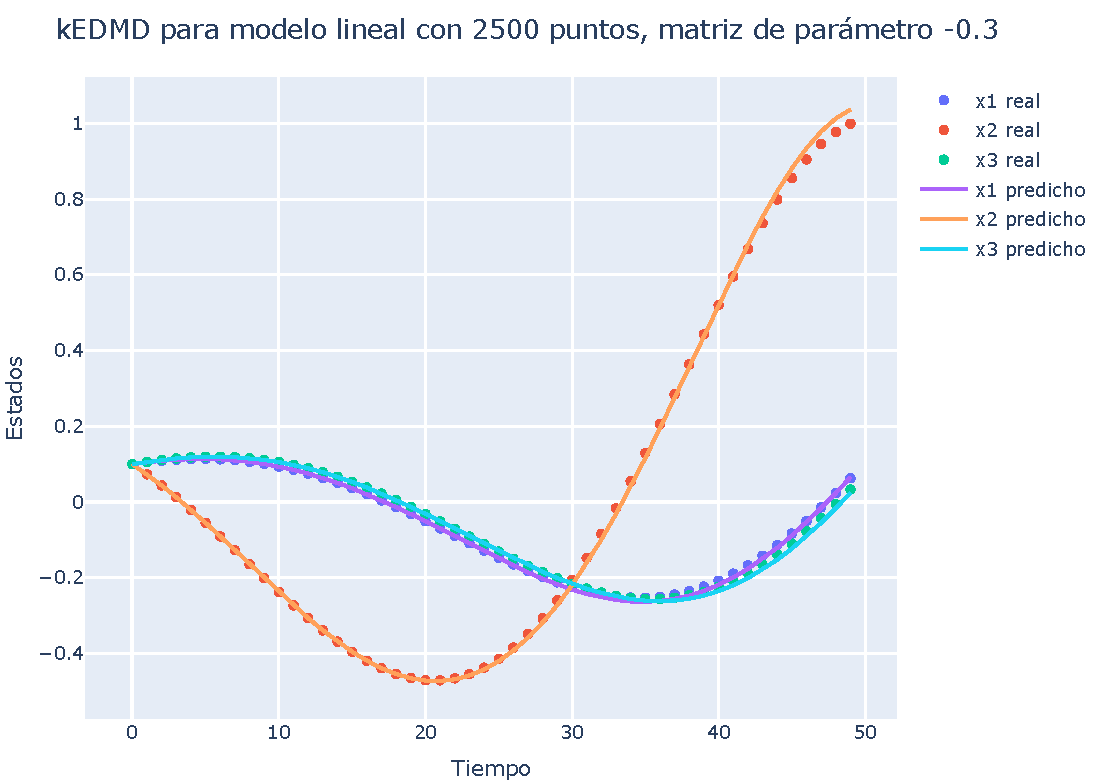
\includegraphics[width=\textwidth]{img/content/chapter3/Linear1.pdf}
        \caption{$\alpha=-0.3$}
        \label{fig:Linear1}
    \end{subfigure}
    \hfill
    \begin{subfigure}[b]{0.32\textwidth}
        \centering
        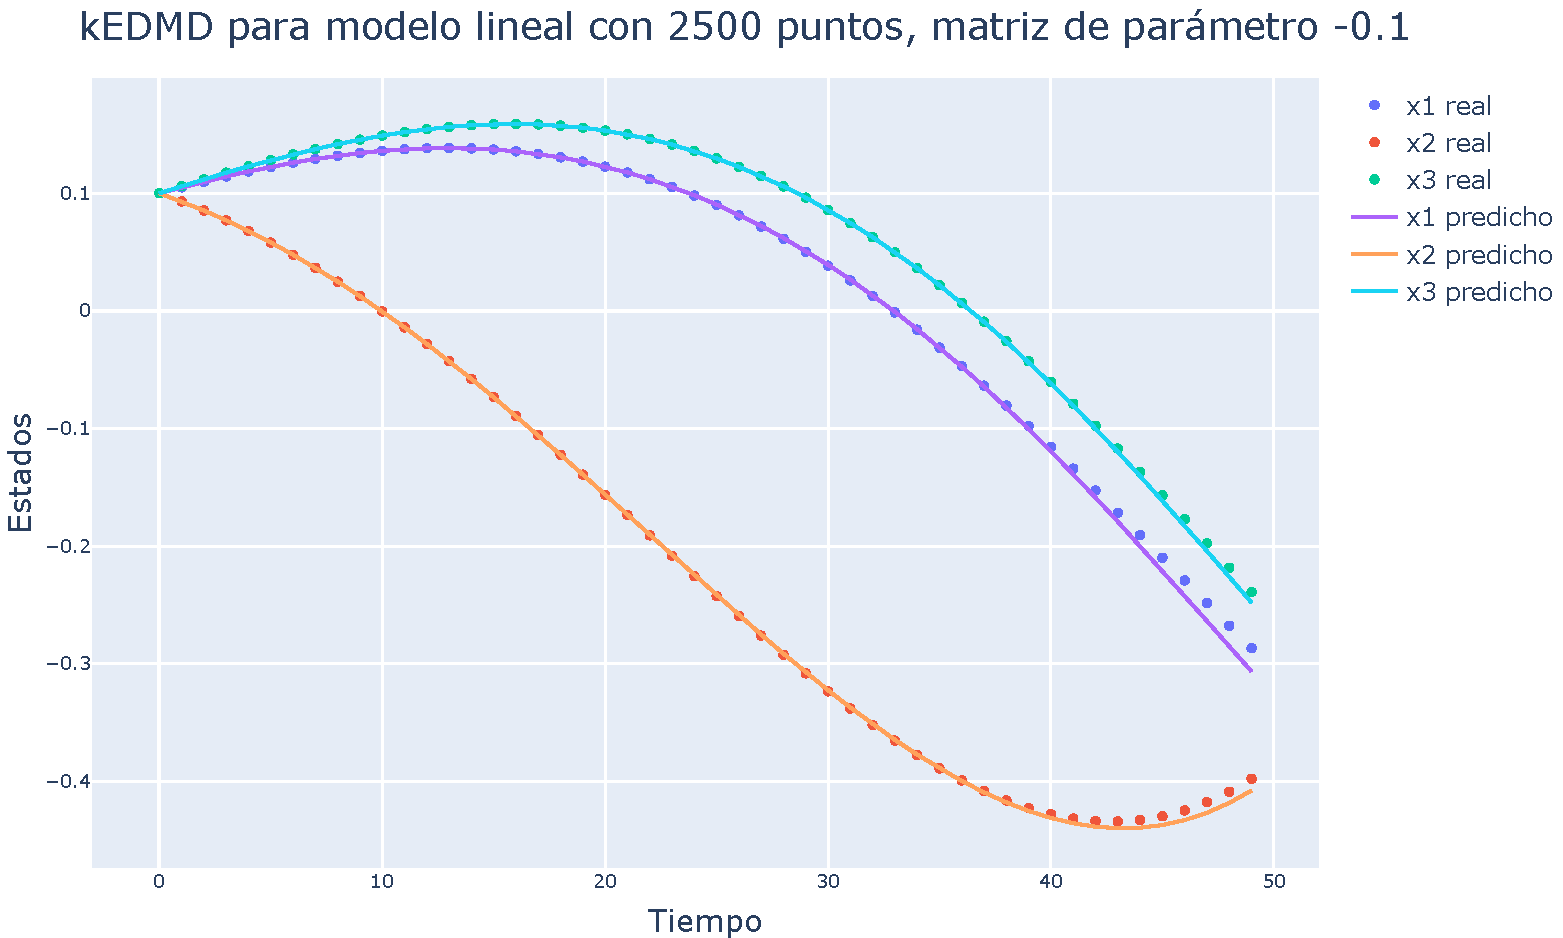
\includegraphics[width=\textwidth]{img/content/chapter3/Linear2.pdf}
        \caption{$\alpha=-0.1$}
        \label{fig:Linear2}
    \end{subfigure}
    \hfill
    \begin{subfigure}[b]{0.32\textwidth}
        \centering
        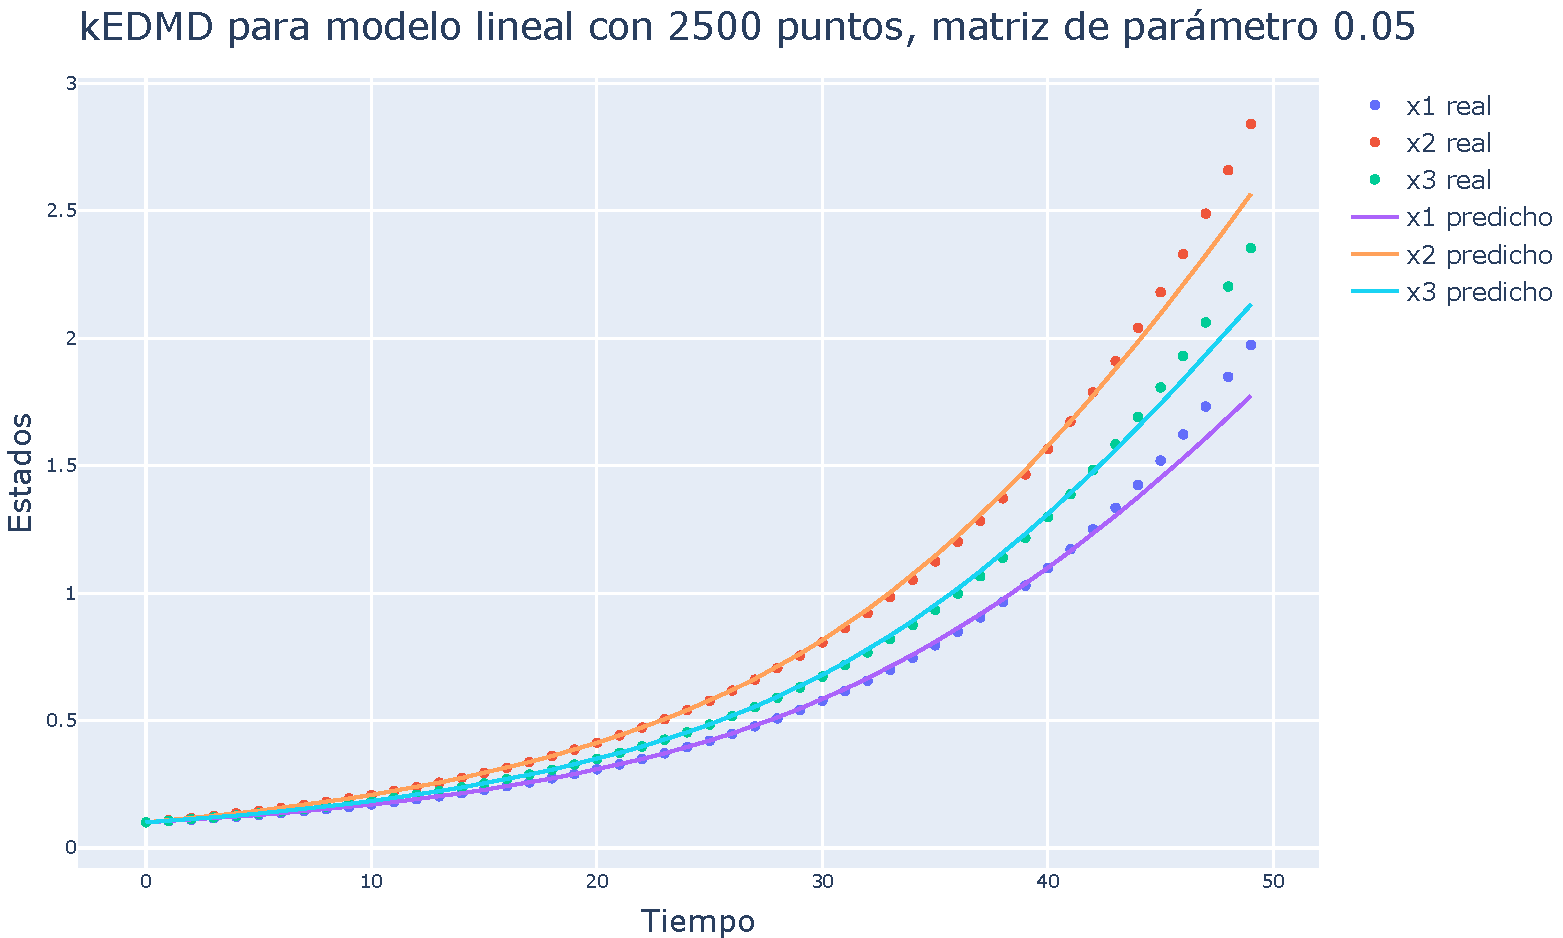
\includegraphics[width=\textwidth]{img/content/chapter3/Linear3.pdf}
        \caption{$\alpha=0.05$}
    \end{subfigure}
    \caption{Ilustración de los tres casos de $\alpha$ elegidos para la comparación entre el sistema lineal original y el sistema linealizado por Koopman a 2500 puntos \textit{sampleados} de una variable aleatoria normal. En forma de puntos se dejan los valores reales que toma el sistema y en línea continua los valores entregados por el sistema linealizado, que se consideran como predicción.}
    \label{fig:Comp_traj_lin}
\end{figure}
Aunque la cota en \eqref{eq:kEDMD_bound} no hace referencia directa a la diferencia en norma de las trayectorias, es de interés analizar el orden en que decae el error en función de $N$, para ello se calcula la diferencia en norma de las trayectorias generadas para $N \in \{ 100k : k \in \{1, \dots, 30\} \}$. 

En la figura \ref{fig:Comp_traj_lin} se observa que las trayectorias obtenidas con el sistema linealizado vía Koopman son muy cercanas a las obtenidas con el sistema lineal original, solo difiriendo en zonas donde el sistema original toma valores muy altos, lo que se puede asociar a la poca probabilidad de \textit{sampleo} que le da la distribución normal elegida a puntos muy alejados del origen. \\
Mientras que en la figura \ref{fig:ErrorLin} se observa que en realidad el orden de decaimiento del error en función de $N$ es mayor que $N^{-1/2}$, mejorando la cota mostrada en \eqref{eq:kEDMD_bound}.
\begin{figure}[h]
    \centering
    \begin{subfigure}[b]{0.32\textwidth}
        \centering
        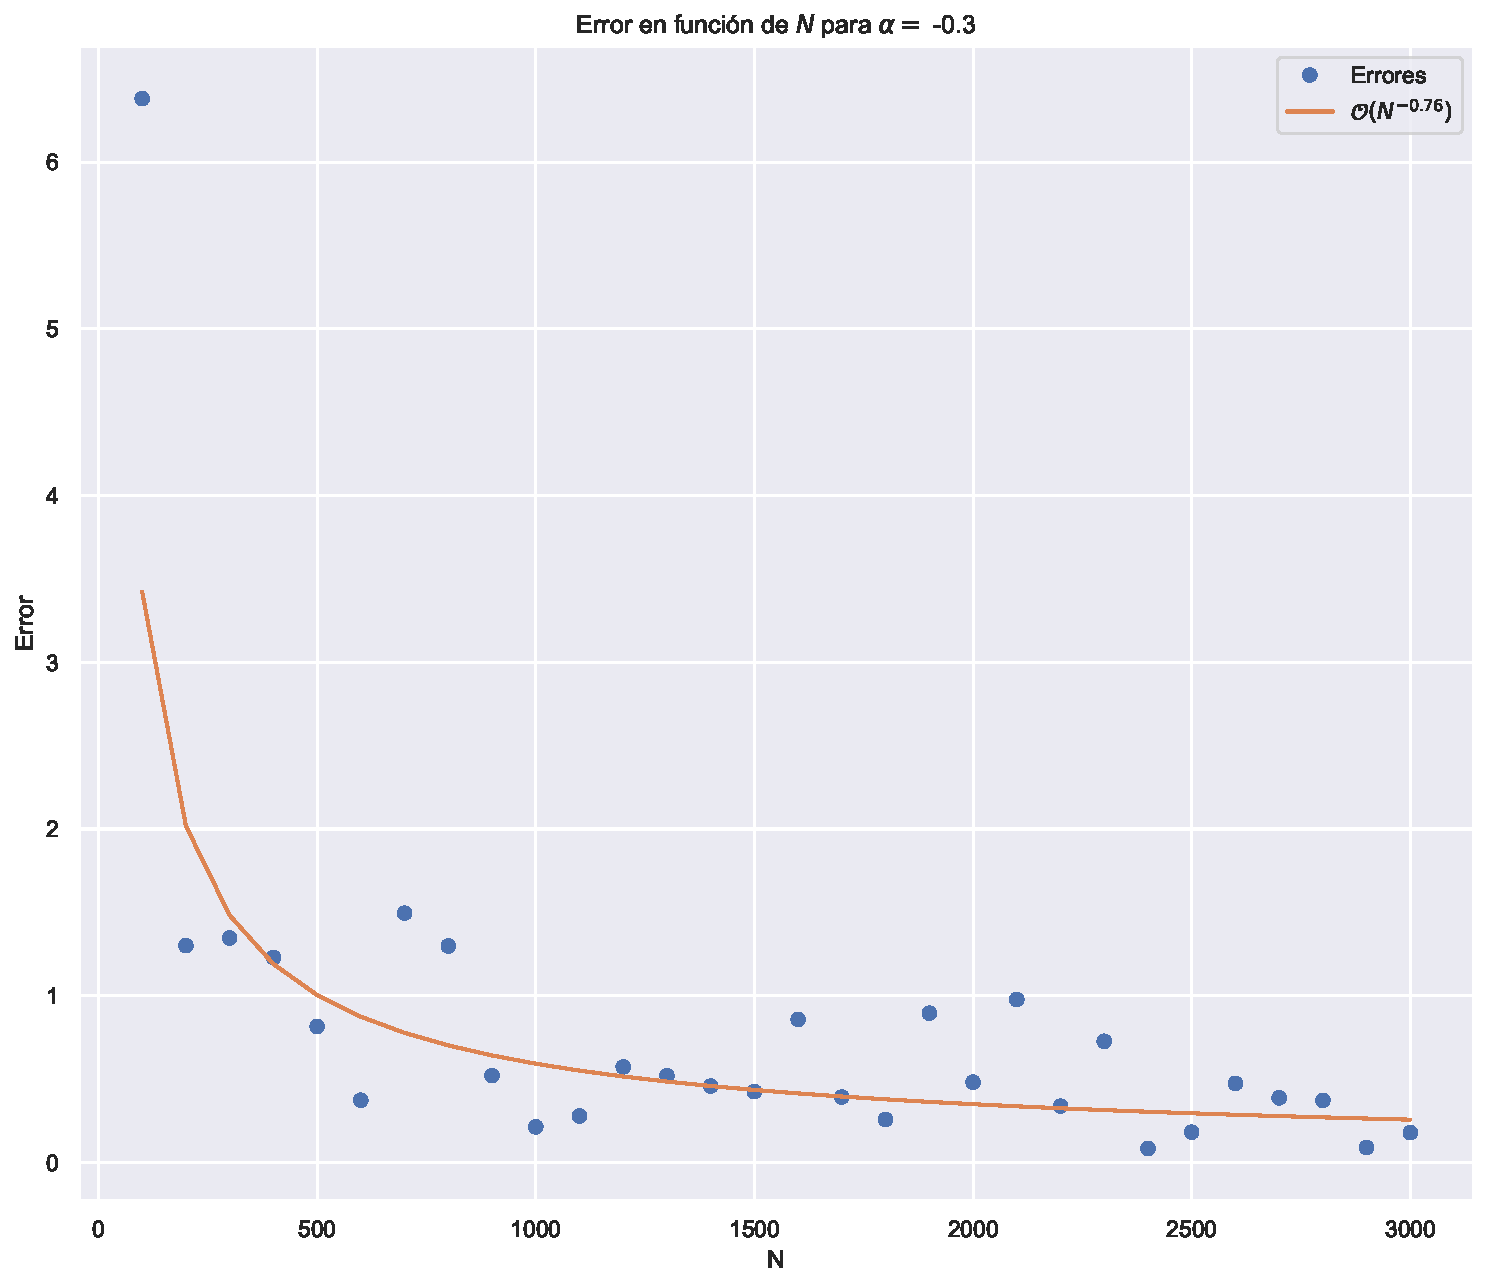
\includegraphics[width=\textwidth]{img/content/chapter3/Linear1Errors.pdf}
        \caption{$\alpha=-0.3$}
        \label{fig:Linear1Errors}
    \end{subfigure}
    \hfill
    \begin{subfigure}[b]{0.32\textwidth}
        \centering
        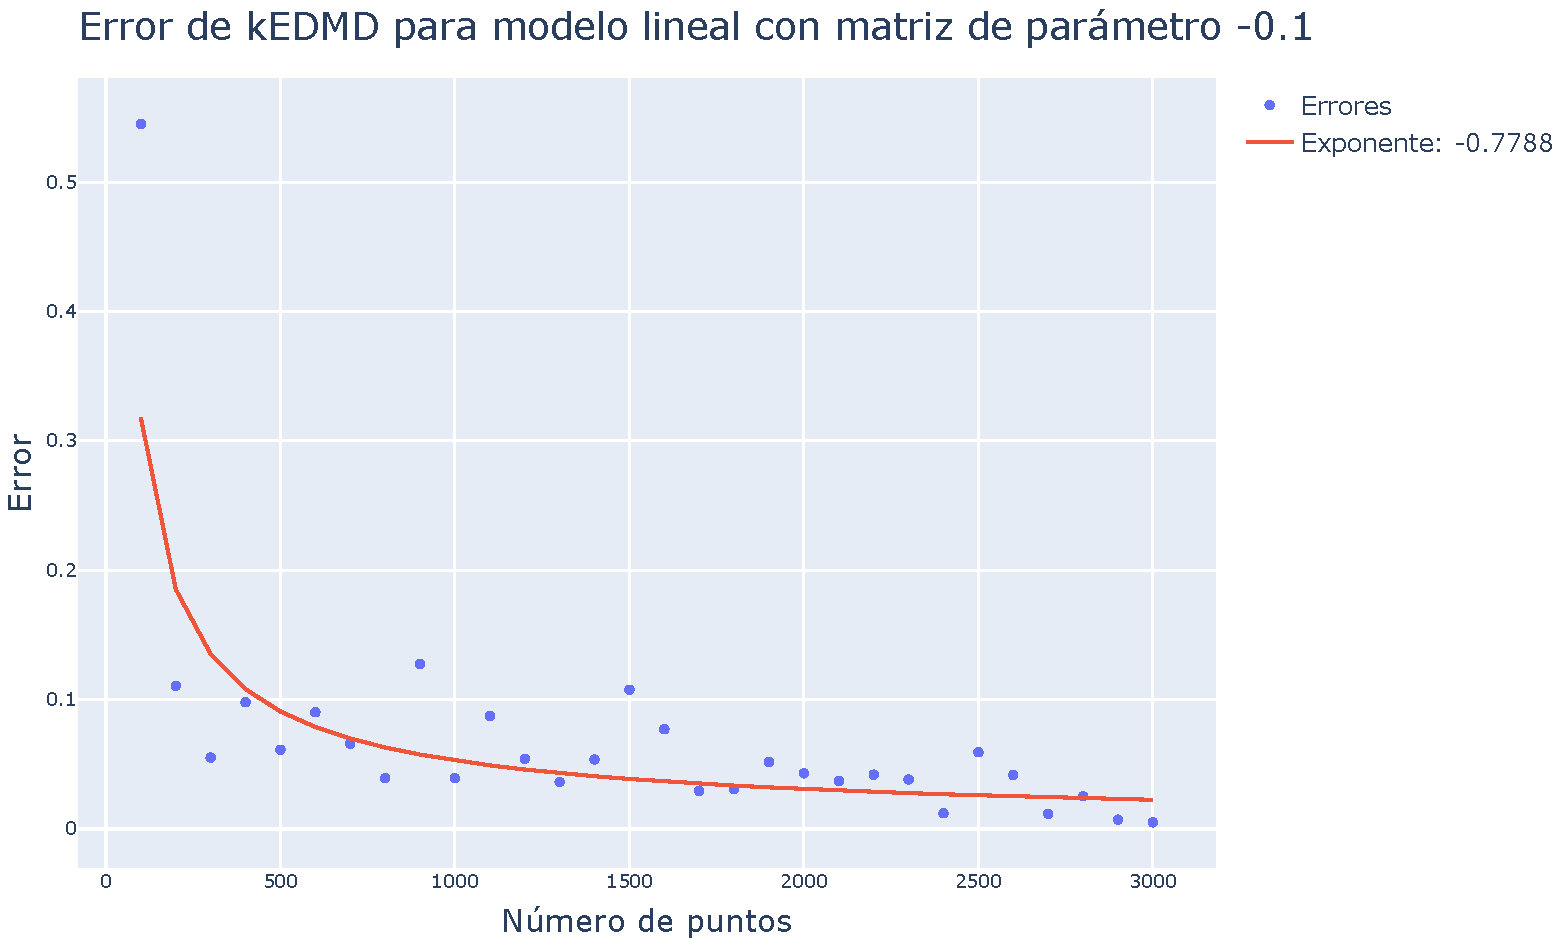
\includegraphics[width=\textwidth]{img/content/chapter3/Linear2Errors.pdf}
        \caption{$\alpha=-0.1$}
        \label{fig:Linear2Errors}
    \end{subfigure}
    \hfill
    \begin{subfigure}[b]{0.32\textwidth}
        \centering
        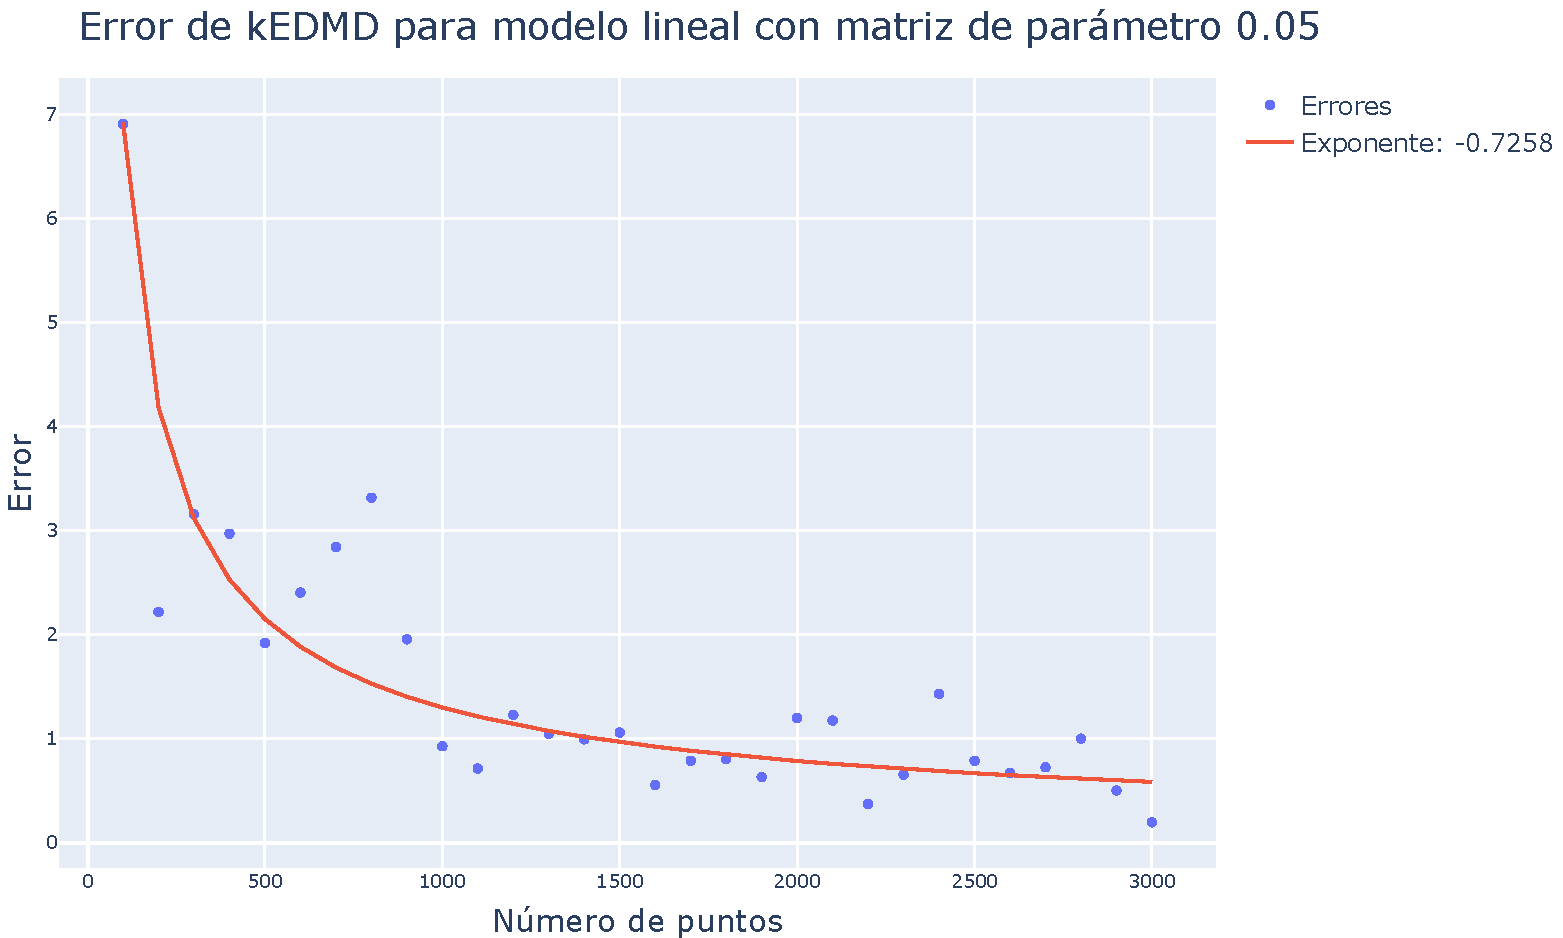
\includegraphics[width=\textwidth]{img/content/chapter3/Linear3Errors.pdf}
        \caption{$\alpha=0.05$}
        \label{fig:image3}
    \end{subfigure}
    \caption{Ilustración de los tres casos de $\alpha$ elegidos para la evolución en función de $N$ de la diferencia en norma entre el sistema lineal original y el sistema linealizado por Koopman a $N$ puntos \textit{sampleados} de una variable aleatoria normal. En forma de puntos se deja la evolución observada del error y en línea continua la mejor curva de la forma $C \cdot N^{a}$, donde $a$ es el exponente que se deja en la leyenda.}
    \label{fig:ErrorLin}
\end{figure}
\subsection{kEDMD para modelos utilizados en epidemiología}
Para esta sección se ilustrarán los resultados de kEDMD para modelos epidemiológicos de tipo SIR y SIRS. Se supondrá que la población está normalizada, esto es, que cada estado está en $[0, 1]$.\\
Dado que no se consideran nacimientos ni muertes, se puede decir que el espacio de estados de este modelo es, sin considerar los eventuales factores estocásticos, un $(n-1)$-simplex, siendo $n$ la cantidad de compartimentos considerados, que se define como el conjunto
\begin{equation*}
    \Delta_{n-1} = \left \{ x \in \R^n : \sum_{i=1}^n x_i = 1, \, x_i \geq 0, \, \forall i \in \{1, \dots, n\} \right \}.
\end{equation*}
De este conjunto se puede \textit{samplear} de manera eficiente desde una distribución Dirichlet \cite{Frigyik2010IntroductionProcesses}, y se encuentra implementado en las principales librerías con funcionalidades estadísticas como SciPy \cite{Virtanen2020SciPyPython}, que será la utilizada en este trabajo.\\
La densidad de una variable aleatoria Dirichlet con parámetros $\alpha_1, \alpha_2, \ldots, \alpha_K$ se define como:
\[
f(x_1, x_2, \ldots, x_K; \alpha_1, \alpha_2, \ldots, \alpha_K) = \frac{1}{B(\alpha)} \prod_{i=1}^{K} x_i^{\alpha_i - 1}
\]
donde $x_i \geq 0$ para todo $i$, $\sum_{i=1}^{K} x_i = 1$, y
\[
B(\alpha) = \frac{\prod_{i=1}^{K} \Gamma(\alpha_i)}{\Gamma\left(\sum_{i=1}^{K} \alpha_i\right)}
\]
es la función beta multivariable, y $\Gamma(\cdot)$ es la función gamma. En la figura \ref{fig:Dirichlet_samples} se puede apreciar la diferencia de \textit{samplear} para diferentes valores de $\alpha$. Un valor de $\alpha$ con entradas iguales genera la misma dispersión en todas las direcciones, siendo $(1, 1, 1)$ la variable aleatoria uniforme en $\Delta_{n-1}$, mientras que valores altos de $\alpha$ generan una alta concentración de muestras en el centro del conjunto. Por otro lado valores desiguales generar mayor cantidad de muestras en alguna de las caras del conjunto.
\begin{figure}[htbp]
    \centering
    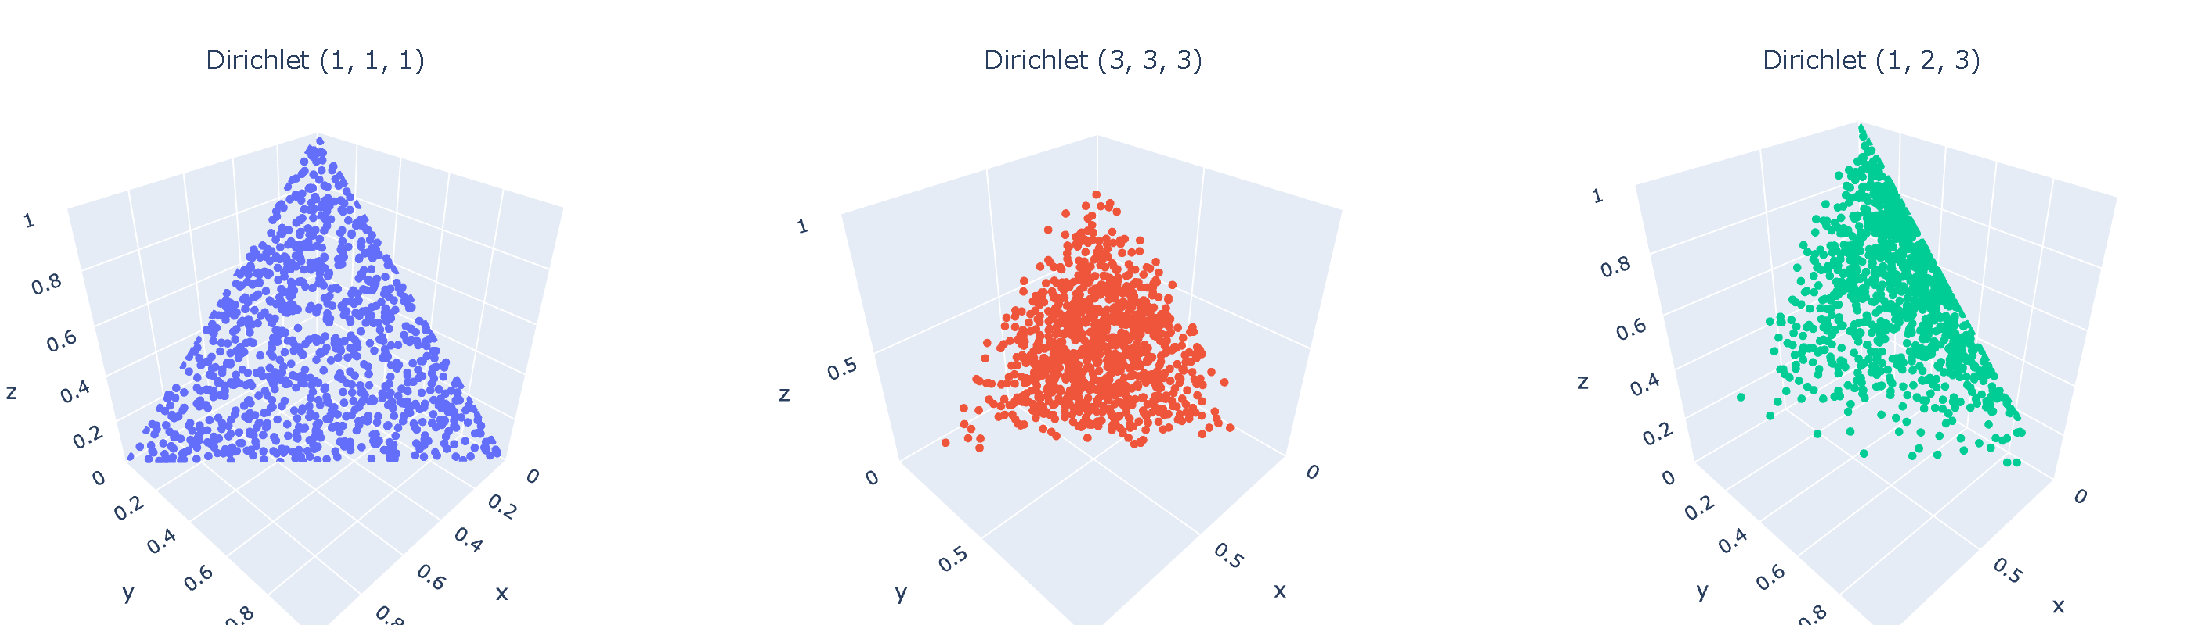
\includegraphics[width=0.95\linewidth]{img/content/chapter3/Dirichlet.pdf}
    \caption{1000 muestras de una variable aleatoria Dirichlet para diferentes valores de $\alpha$, observando dos casos de $\alpha$ con valores homogéneos y uno con valores heterogéneos, lo que provoca un desbalance de muestras.}
    \label{fig:Dirichlet_samples}
\end{figure}

Se visualizará la aproximación por kEDMD para los modelos SIR y SIRS, con la misma configuración en común, salvo, obviamente, el parámetro $\alpha$ correspondiente al segundo modelo. Se utilizó \textit{kernel} de Matérn de parámetro $\nu=1/2$ y ancho de banda $\gamma=10^{-3}$. Se utiliza una distribución Dirichlet de parámetro $(1,1,1)$ como variable aleatoria asociada al espacio de estados y ruido aditivo centrado y Gaussiano de matriz de covarianza $10^{-7} I_{3 \times 3}$, de estas distribuciones se \textit{samplearán} $N=1000$ puntos. Se toma como condición inicial $\mathbf{x}_0 = (0.9, 0.1, 0.0)$ y los resultados obtenidos se pueden ver en las figuras \ref{fig:Comp_traj_SIR} y \ref{fig:Comp_traj_SIRS}. 

Similar a lo hecho en el caso lineal, en las figuras \ref{fig:ErrorSIR} y \ref{fig:ErrorSIRS} se comparan las diferencias en norma entre las trayectorias originales y las trayectoria linealizadas, con la mejor curva de la forma $C \cdot N^{a}$, para observar si los errores andan en el orden de decaimiento en \eqref{eq:kEDMD_bound}.

Se observa nuevamente que la discrepancia entre las trayectorias en efecto anda del orden de la cota expuesta en este capítulo, incluso con decaimientos aún más rápidos.

Se comparan las trayectorias generadas por el sistema original con las generadas por kEDMD, utilizando exactamente la misma configuración del sistema anterior, solo cambiando la dinámica.

Nuevamente se observa que el orden de discrepancia de las trayectorias es de un orden similar, o incluso menor, al visto en la cota \ref{eq:kEDMD_bound}.